\documentclass[1p]{elsarticle_modified}
%\bibliographystyle{elsarticle-num}

%\usepackage[colorlinks]{hyperref}
%\usepackage{abbrmath_seonhwa} %\Abb, \Ascr, \Acal ,\Abf, \Afrak
\usepackage{amsfonts}
\usepackage{amssymb}
\usepackage{amsmath}
\usepackage{amsthm}
\usepackage{scalefnt}
\usepackage{amsbsy}
\usepackage{kotex}
\usepackage{caption}
\usepackage{subfig}
\usepackage{color}
\usepackage{graphicx}
\usepackage{xcolor} %% white, black, red, green, blue, cyan, magenta, yellow
\usepackage{float}
\usepackage{setspace}
\usepackage{hyperref}

\usepackage{tikz}
\usetikzlibrary{arrows}

\usepackage{multirow}
\usepackage{array} % fixed length table
\usepackage{hhline}

%%%%%%%%%%%%%%%%%%%%%
\makeatletter
\renewcommand*\env@matrix[1][\arraystretch]{%
	\edef\arraystretch{#1}%
	\hskip -\arraycolsep
	\let\@ifnextchar\new@ifnextchar
	\array{*\c@MaxMatrixCols c}}
\makeatother %https://tex.stackexchange.com/questions/14071/how-can-i-increase-the-line-spacing-in-a-matrix
%%%%%%%%%%%%%%%

\usepackage[normalem]{ulem}

\newcommand{\msout}[1]{\ifmmode\text{\sout{\ensuremath{#1}}}\else\sout{#1}\fi}
%SOURCE: \msout is \stkout macro in https://tex.stackexchange.com/questions/20609/strikeout-in-math-mode

\newcommand{\cancel}[1]{
	\ifmmode
	{\color{red}\msout{#1}}
	\else
	{\color{red}\sout{#1}}
	\fi
}

\newcommand{\add}[1]{
	{\color{blue}\uwave{#1}}
}

\newcommand{\replace}[2]{
	\ifmmode
	{\color{red}\msout{#1}}{\color{blue}\uwave{#2}}
	\else
	{\color{red}\sout{#1}}{\color{blue}\uwave{#2}}
	\fi
}

\newcommand{\Sol}{\mathcal{S}} %segment
\newcommand{\D}{D} %diagram
\newcommand{\A}{\mathcal{A}} %arc


%%%%%%%%%%%%%%%%%%%%%%%%%%%%%5 test

\def\sl{\operatorname{\textup{SL}}(2,\Cbb)}
\def\psl{\operatorname{\textup{PSL}}(2,\Cbb)}
\def\quan{\mkern 1mu \triangleright \mkern 1mu}

\theoremstyle{definition}
\newtheorem{thm}{Theorem}[section]
\newtheorem{prop}[thm]{Proposition}
\newtheorem{lem}[thm]{Lemma}
\newtheorem{ques}[thm]{Question}
\newtheorem{cor}[thm]{Corollary}
\newtheorem{defn}[thm]{Definition}
\newtheorem{exam}[thm]{Example}
\newtheorem{rmk}[thm]{Remark}
\newtheorem{alg}[thm]{Algorithm}

\newcommand{\I}{\sqrt{-1}}
\begin{document}

%\begin{frontmatter}
%
%\title{Boundary parabolic representations of knots up to 8 crossings}
%
%%% Group authors per affiliation:
%\author{Yunhi Cho} 
%\address{Department of Mathematics, University of Seoul, Seoul, Korea}
%\ead{yhcho@uos.ac.kr}
%
%
%\author{Seonhwa Kim} %\fnref{s_kim}}
%\address{Center for Geometry and Physics, Institute for Basic Science, Pohang, 37673, Korea}
%\ead{ryeona17@ibs.re.kr}
%
%\author{Hyuk Kim}
%\address{Department of Mathematical Sciences, Seoul National University, Seoul 08826, Korea}
%\ead{hyukkim@snu.ac.kr}
%
%\author{Seokbeom Yoon}
%\address{Department of Mathematical Sciences, Seoul National University, Seoul, 08826,  Korea}
%\ead{sbyoon15@snu.ac.kr}
%
%\begin{abstract}
%We find all boundary parabolic representation of knots up to 8 crossings.
%
%\end{abstract}
%\begin{keyword}
%    \MSC[2010] 57M25 
%\end{keyword}
%
%\end{frontmatter}

%\linenumbers
%\tableofcontents
%
\newcommand\colored[1]{\textcolor{white}{\rule[-0.35ex]{0.8em}{1.4ex}}\kern-0.8em\color{red} #1}%
%\newcommand\colored[1]{\textcolor{white}{ #1}\kern-2.17ex	\textcolor{white}{ #1}\kern-1.81ex	\textcolor{white}{ #1}\kern-2.15ex\color{red}#1	}

{\Large $\underline{12a_{1088}~(K12a_{1088})}$}

\setlength{\tabcolsep}{10pt}
\renewcommand{\arraystretch}{1.6}
\vspace{1cm}\begin{tabular}{m{100pt}>{\centering\arraybackslash}m{274pt}}
\multirow{5}{120pt}{
	\centering
	\includegraphics[width=112pt]{../../../GIT/diagram.site/Diagrams/png/1889_12a_1088.png}\\
\ \ \ A knot diagram\footnotemark}&
\allowdisplaybreaks
\textbf{Linearized knot diagam} \\
\cline{2-2}
 &
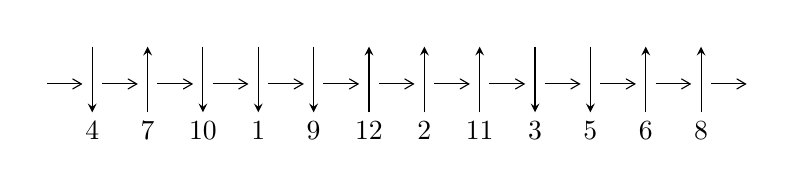
\begin{tikzpicture}[x=20pt, y=17pt]
	% nodes
	\node (C0) at (0, 0) {};
	\node (C1) at (1, 0) {};
	\node (C1U) at (1, +1) {};
	\node (C1D) at (1, -1) {4};

	\node (C2) at (2, 0) {};
	\node (C2U) at (2, +1) {};
	\node (C2D) at (2, -1) {7};

	\node (C3) at (3, 0) {};
	\node (C3U) at (3, +1) {};
	\node (C3D) at (3, -1) {10};

	\node (C4) at (4, 0) {};
	\node (C4U) at (4, +1) {};
	\node (C4D) at (4, -1) {1};

	\node (C5) at (5, 0) {};
	\node (C5U) at (5, +1) {};
	\node (C5D) at (5, -1) {9};

	\node (C6) at (6, 0) {};
	\node (C6U) at (6, +1) {};
	\node (C6D) at (6, -1) {12};

	\node (C7) at (7, 0) {};
	\node (C7U) at (7, +1) {};
	\node (C7D) at (7, -1) {2};

	\node (C8) at (8, 0) {};
	\node (C8U) at (8, +1) {};
	\node (C8D) at (8, -1) {11};

	\node (C9) at (9, 0) {};
	\node (C9U) at (9, +1) {};
	\node (C9D) at (9, -1) {3};

	\node (C10) at (10, 0) {};
	\node (C10U) at (10, +1) {};
	\node (C10D) at (10, -1) {5};

	\node (C11) at (11, 0) {};
	\node (C11U) at (11, +1) {};
	\node (C11D) at (11, -1) {6};

	\node (C12) at (12, 0) {};
	\node (C12U) at (12, +1) {};
	\node (C12D) at (12, -1) {8};
	\node (C13) at (13, 0) {};

	% arrows
	\draw[->,>={angle 60}]
	(C0) edge (C1) (C1) edge (C2) (C2) edge (C3) (C3) edge (C4) (C4) edge (C5) (C5) edge (C6) (C6) edge (C7) (C7) edge (C8) (C8) edge (C9) (C9) edge (C10) (C10) edge (C11) (C11) edge (C12) (C12) edge (C13) ;	\draw[->,>=stealth]
	(C1U) edge (C1D) (C2D) edge (C2U) (C3U) edge (C3D) (C4U) edge (C4D) (C5U) edge (C5D) (C6D) edge (C6U) (C7D) edge (C7U) (C8D) edge (C8U) (C9U) edge (C9D) (C10U) edge (C10D) (C11D) edge (C11U) (C12D) edge (C12U) ;
	\end{tikzpicture} \\
\hhline{~~} \\& 
\textbf{Solving Sequence} \\ \cline{2-2} 
 &
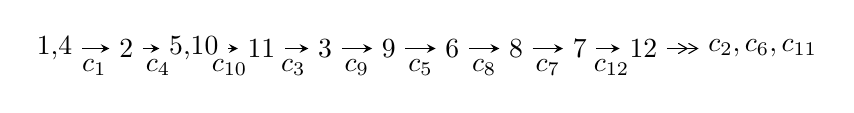
\begin{tikzpicture}[x=23pt, y=7pt]
	% node
	\node (A0) at (-1/8, 0) {1,4};
	\node (A1) at (1, 0) {2};
	\node (A2) at (33/16, 0) {5,10};
	\node (A3) at (25/8, 0) {11};
	\node (A4) at (33/8, 0) {3};
	\node (A5) at (41/8, 0) {9};
	\node (A6) at (49/8, 0) {6};
	\node (A7) at (57/8, 0) {8};
	\node (A8) at (65/8, 0) {7};
	\node (A9) at (73/8, 0) {12};
	\node (C1) at (1/2, -1) {$c_{1}$};
	\node (C2) at (3/2, -1) {$c_{4}$};
	\node (C3) at (21/8, -1) {$c_{10}$};
	\node (C4) at (29/8, -1) {$c_{3}$};
	\node (C5) at (37/8, -1) {$c_{9}$};
	\node (C6) at (45/8, -1) {$c_{5}$};
	\node (C7) at (53/8, -1) {$c_{8}$};
	\node (C8) at (61/8, -1) {$c_{7}$};
	\node (C9) at (69/8, -1) {$c_{12}$};
	\node (A10) at (11, 0) {$c_{2},c_{6},c_{11}$};

	% edge
	\draw[->,>=stealth]	
	(A0) edge (A1) (A1) edge (A2) (A2) edge (A3) (A3) edge (A4) (A4) edge (A5) (A5) edge (A6) (A6) edge (A7) (A7) edge (A8) (A8) edge (A9) ;
	\draw[->>,>={angle 60}]	
	(A9) edge (A10);
\end{tikzpicture} \\ 

\end{tabular} \\

\footnotetext{
The image of knot diagram is generated by the software ``\textbf{Draw programme}" developed by Andrew Bartholomew(\url{http://www.layer8.co.uk/maths/draw/index.htm\#Running-draw}), where we modified some parts for our purpose(\url{https://github.com/CATsTAILs/LinksPainter}).
}\phantom \\ \newline 
\centering \textbf{Ideals for irreducible components\footnotemark of $X_{\text{par}}$} 
 
\begin{align*}
I^u_{1}&=\langle 
2.31491\times10^{1036} u^{173}+1.57790\times10^{1037} u^{172}+\cdots+3.00068\times10^{1038} b+2.78340\times10^{1039},\\
\phantom{I^u_{1}}&\phantom{= \langle  }-1.81611\times10^{1038} u^{173}-1.79120\times10^{1039} u^{172}+\cdots+3.69384\times10^{1041} a-1.30081\times10^{1043},\\
\phantom{I^u_{1}}&\phantom{= \langle  }u^{174}+7 u^{173}+\cdots+32468 u+1231\rangle \\
I^u_{2}&=\langle 
-7.43715\times10^{54} u^{47}+3.00397\times10^{55} u^{46}+\cdots+1.20510\times10^{53} b-5.50344\times10^{54},\\
\phantom{I^u_{2}}&\phantom{= \langle  }4.76026\times10^{54} u^{47}-2.21701\times10^{55} u^{46}+\cdots+1.20510\times10^{53} a-9.61062\times10^{54},\;u^{48}-4 u^{47}+\cdots+3 u+1\rangle \\
\\
\end{align*}
\raggedright * 2 irreducible components of $\dim_{\mathbb{C}}=0$, with total 222 representations.\\
\footnotetext{All coefficients of polynomials are rational numbers. But the coefficients are sometimes approximated in decimal forms when there is not enough margin.}
\newpage
\renewcommand{\arraystretch}{1}
\centering \section*{I. $I^u_{1}= \langle 2.31\times10^{1036} u^{173}+1.58\times10^{1037} u^{172}+\cdots+3.00\times10^{1038} b+2.78\times10^{1039},\;-1.82\times10^{1038} u^{173}-1.79\times10^{1039} u^{172}+\cdots+3.69\times10^{1041} a-1.30\times10^{1043},\;u^{174}+7 u^{173}+\cdots+32468 u+1231 \rangle$}
\flushleft \textbf{(i) Arc colorings}\\
\begin{tabular}{m{7pt} m{180pt} m{7pt} m{180pt} }
\flushright $a_{1}=$&$\begin{pmatrix}1\\0\end{pmatrix}$ \\
\flushright $a_{4}=$&$\begin{pmatrix}0\\u\end{pmatrix}$ \\
\flushright $a_{2}=$&$\begin{pmatrix}1\\u^2\end{pmatrix}$ \\
\flushright $a_{5}=$&$\begin{pmatrix}- u\\u\end{pmatrix}$ \\
\flushright $a_{10}=$&$\begin{pmatrix}0.000491659 u^{173}+0.00484915 u^{172}+\cdots+644.740 u+35.2157\\-0.00771462 u^{173}-0.0525848 u^{172}+\cdots-283.377 u-9.27589\end{pmatrix}$ \\
\flushright $a_{11}=$&$\begin{pmatrix}-0.00428694 u^{173}-0.0237318 u^{172}+\cdots+727.574 u+38.6934\\-0.00293603 u^{173}-0.0240038 u^{172}+\cdots-366.211 u-12.7536\end{pmatrix}$ \\
\flushright $a_{3}=$&$\begin{pmatrix}0.00331237 u^{173}+0.0263307 u^{172}+\cdots-13.6765 u-9.11805\\-0.00830572 u^{173}-0.0573603 u^{172}+\cdots-199.908 u-7.28134\end{pmatrix}$ \\
\flushright $a_{9}=$&$\begin{pmatrix}0.000473903 u^{173}-0.00172132 u^{172}+\cdots-234.484 u-4.16866\\-0.00269431 u^{173}-0.0157973 u^{172}+\cdots-45.6029 u-1.40926\end{pmatrix}$ \\
\flushright $a_{6}=$&$\begin{pmatrix}-0.0219404 u^{173}-0.151654 u^{172}+\cdots-303.429 u-6.94477\\0.0114226 u^{173}+0.0765005 u^{172}+\cdots-28.4166 u-3.12707\end{pmatrix}$ \\
\flushright $a_{8}=$&$\begin{pmatrix}-0.0118555 u^{173}-0.0795581 u^{172}+\cdots+449.141 u+33.2239\\0.00484708 u^{173}+0.0315881 u^{172}+\cdots+109.574 u+4.82128\end{pmatrix}$ \\
\flushright $a_{7}=$&$\begin{pmatrix}-0.0133040 u^{173}-0.0899921 u^{172}+\cdots+242.794 u+24.1803\\0.00536885 u^{173}+0.0348291 u^{172}+\cdots+120.908 u+5.18340\end{pmatrix}$ \\
\flushright $a_{12}=$&$\begin{pmatrix}-0.0231211 u^{173}-0.148324 u^{172}+\cdots+623.503 u+40.0407\\0.00823559 u^{173}+0.0513008 u^{172}+\cdots-209.974 u-9.11274\end{pmatrix}$\\&\end{tabular}
\flushleft \textbf{(ii) Obstruction class $= -1$}\\~\\
\flushleft \textbf{(iii) Cusp Shapes $= 0.00680530 u^{173}+0.0466019 u^{172}+\cdots+155.904 u+9.18362$}\\~\\
\newpage\renewcommand{\arraystretch}{1}
\flushleft \textbf{(iv) u-Polynomials at the component}\newline \\
\begin{tabular}{m{50pt}|m{274pt}}
Crossings & \hspace{64pt}u-Polynomials at each crossing \\
\hline $$\begin{aligned}c_{1},c_{4}\end{aligned}$$&$\begin{aligned}
&u^{174}-7 u^{173}+\cdots-32468 u+1231
\end{aligned}$\\
\hline $$\begin{aligned}c_{2},c_{7}\end{aligned}$$&$\begin{aligned}
&9(9 u^{174}+21 u^{173}+\cdots+57344 u+284672)
\end{aligned}$\\
\hline $$\begin{aligned}c_{3},c_{9}\end{aligned}$$&$\begin{aligned}
&9(9 u^{174}+21 u^{173}+\cdots+5.26430\times10^{7} u+7135679)
\end{aligned}$\\
\hline $$\begin{aligned}c_{5}\end{aligned}$$&$\begin{aligned}
&u^{174}+7 u^{173}+\cdots-115375851 u+8331579
\end{aligned}$\\
\hline $$\begin{aligned}c_{6},c_{11}\end{aligned}$$&$\begin{aligned}
&u^{174}+8 u^{173}+\cdots+103307 u+4271
\end{aligned}$\\
\hline $$\begin{aligned}c_{8}\end{aligned}$$&$\begin{aligned}
&81(81 u^{174}+1989 u^{173}+\cdots+432 u+32)
\end{aligned}$\\
\hline $$\begin{aligned}c_{10}\end{aligned}$$&$\begin{aligned}
&u^{174}-14 u^{172}+\cdots+207068871 u+14948811
\end{aligned}$\\
\hline $$\begin{aligned}c_{12}\end{aligned}$$&$\begin{aligned}
&u^{174}-3 u^{173}+\cdots+502185 u+36513
\end{aligned}$\\
\hline
\end{tabular}\\~\\
\newpage\renewcommand{\arraystretch}{1}
\flushleft \textbf{(v) Riley Polynomials at the component}\newline \\
\begin{tabular}{m{50pt}|m{274pt}}
Crossings & \hspace{64pt}Riley Polynomials at each crossing \\
\hline $$\begin{aligned}c_{1},c_{4}\end{aligned}$$&$\begin{aligned}
&y^{174}+85 y^{173}+\cdots+414366 y+1515361
\end{aligned}$\\
\hline $$\begin{aligned}c_{2},c_{7}\end{aligned}$$&$\begin{aligned}
&81(81 y^{174}+7083 y^{173}+\cdots+4.33429\times10^{12} y+8.10381\times10^{10})
\end{aligned}$\\
\hline $$\begin{aligned}c_{3},c_{9}\end{aligned}$$&$\begin{aligned}
&81\\
&\cdot(81 y^{174}-9279 y^{173}+\cdots-2842222453168320 y+50917914791041)
\end{aligned}$\\
\hline $$\begin{aligned}c_{5}\end{aligned}$$&$\begin{aligned}
&y^{174}+29 y^{173}+\cdots+23467085991243 y+69415208633241
\end{aligned}$\\
\hline $$\begin{aligned}c_{6},c_{11}\end{aligned}$$&$\begin{aligned}
&y^{174}-122 y^{173}+\cdots+2710884961 y+18241441
\end{aligned}$\\
\hline $$\begin{aligned}c_{8}\end{aligned}$$&$\begin{aligned}
&6561(6561 y^{174}-480573 y^{173}+\cdots-84736 y+1024)
\end{aligned}$\\
\hline $$\begin{aligned}c_{10}\end{aligned}$$&$\begin{aligned}
&y^{174}-28 y^{173}+\cdots-12744162723038499 y+223466950313721
\end{aligned}$\\
\hline $$\begin{aligned}c_{12}\end{aligned}$$&$\begin{aligned}
&y^{174}-13 y^{173}+\cdots+591008001867 y+1333199169
\end{aligned}$\\
\hline
\end{tabular}\\~\\
\newpage\flushleft \textbf{(vi) Complex Volumes and Cusp Shapes}
$$\begin{array}{c|c|c}  
\text{Solutions to }I^u_{1}& \I (\text{vol} + \sqrt{-1}CS) & \text{Cusp shape}\\
 \hline 
\begin{aligned}
u &= \phantom{-}0.013817 + 1.000970 I \\
a &= -0.877606 + 0.723543 I \\
b &= \phantom{-}0.975979 - 0.832856 I\end{aligned}
 & \phantom{-}3.55650 - 4.85750 I & \phantom{-0.000000 } 0 \\ \hline\begin{aligned}
u &= \phantom{-}0.013817 - 1.000970 I \\
a &= -0.877606 - 0.723543 I \\
b &= \phantom{-}0.975979 + 0.832856 I\end{aligned}
 & \phantom{-}3.55650 + 4.85750 I & \phantom{-0.000000 } 0 \\ \hline\begin{aligned}
u &= -0.336662 + 0.936143 I \\
a &= \phantom{-}0.622357 + 0.926294 I \\
b &= -2.14550 - 2.04462 I\end{aligned}
 & -5.69350 + 2.20256 I & \phantom{-0.000000 } 0 \\ \hline\begin{aligned}
u &= -0.336662 - 0.936143 I \\
a &= \phantom{-}0.622357 - 0.926294 I \\
b &= -2.14550 + 2.04462 I\end{aligned}
 & -5.69350 - 2.20256 I & \phantom{-0.000000 } 0 \\ \hline\begin{aligned}
u &= \phantom{-}0.492686 + 0.861147 I \\
a &= \phantom{-}0.70963 - 2.34362 I \\
b &= -0.76003 + 1.86058 I\end{aligned}
 & \phantom{-}1.69785 - 2.03628 I & \phantom{-0.000000 } 0 \\ \hline\begin{aligned}
u &= \phantom{-}0.492686 - 0.861147 I \\
a &= \phantom{-}0.70963 + 2.34362 I \\
b &= -0.76003 - 1.86058 I\end{aligned}
 & \phantom{-}1.69785 + 2.03628 I & \phantom{-0.000000 } 0 \\ \hline\begin{aligned}
u &= \phantom{-}0.447668 + 0.885202 I \\
a &= -1.16858 + 1.26192 I \\
b &= \phantom{-}1.79422 - 1.04409 I\end{aligned}
 & \phantom{-}1.75392 - 1.84767 I & \phantom{-0.000000 } 0 \\ \hline\begin{aligned}
u &= \phantom{-}0.447668 - 0.885202 I \\
a &= -1.16858 - 1.26192 I \\
b &= \phantom{-}1.79422 + 1.04409 I\end{aligned}
 & \phantom{-}1.75392 + 1.84767 I & \phantom{-0.000000 } 0 \\ \hline\begin{aligned}
u &= \phantom{-}0.328880 + 0.961073 I \\
a &= \phantom{-}0.605411 - 0.853636 I \\
b &= -2.18230 - 0.61609 I\end{aligned}
 & \phantom{-}5.11610 - 3.70241 I & \phantom{-0.000000 } 0 \\ \hline\begin{aligned}
u &= \phantom{-}0.328880 - 0.961073 I \\
a &= \phantom{-}0.605411 + 0.853636 I \\
b &= -2.18230 + 0.61609 I\end{aligned}
 & \phantom{-}5.11610 + 3.70241 I & \phantom{-0.000000 } 0\\
 \hline 
 \end{array}$$\newpage$$\begin{array}{c|c|c}  
\text{Solutions to }I^u_{1}& \I (\text{vol} + \sqrt{-1}CS) & \text{Cusp shape}\\
 \hline 
\begin{aligned}
u &= \phantom{-}0.955094 + 0.233275 I \\
a &= \phantom{-}1.128060 - 0.703433 I \\
b &= -0.133729 - 0.261612 I\end{aligned}
 & \phantom{-}0.25760 + 8.11693 I & \phantom{-0.000000 } 0 \\ \hline\begin{aligned}
u &= \phantom{-}0.955094 - 0.233275 I \\
a &= \phantom{-}1.128060 + 0.703433 I \\
b &= -0.133729 + 0.261612 I\end{aligned}
 & \phantom{-}0.25760 - 8.11693 I & \phantom{-0.000000 } 0 \\ \hline\begin{aligned}
u &= \phantom{-}0.406624 + 0.895025 I \\
a &= -1.17116 - 0.81104 I \\
b &= \phantom{-}1.64239 + 0.37068 I\end{aligned}
 & \phantom{-}0.87176 - 1.68280 I & \phantom{-0.000000 } 0 \\ \hline\begin{aligned}
u &= \phantom{-}0.406624 - 0.895025 I \\
a &= -1.17116 + 0.81104 I \\
b &= \phantom{-}1.64239 - 0.37068 I\end{aligned}
 & \phantom{-}0.87176 + 1.68280 I & \phantom{-0.000000 } 0 \\ \hline\begin{aligned}
u &= -0.738781 + 0.646428 I \\
a &= -1.092200 - 0.648075 I \\
b &= \phantom{-}0.390019 - 0.380217 I\end{aligned}
 & -2.65819 + 6.17258 I & \phantom{-0.000000 } 0 \\ \hline\begin{aligned}
u &= -0.738781 - 0.646428 I \\
a &= -1.092200 + 0.648075 I \\
b &= \phantom{-}0.390019 + 0.380217 I\end{aligned}
 & -2.65819 - 6.17258 I & \phantom{-0.000000 } 0 \\ \hline\begin{aligned}
u &= -0.810447 + 0.546598 I \\
a &= -0.69029 - 1.24742 I \\
b &= \phantom{-}0.325194 + 0.260356 I\end{aligned}
 & -2.12549 - 5.85975 I & \phantom{-0.000000 } 0 \\ \hline\begin{aligned}
u &= -0.810447 - 0.546598 I \\
a &= -0.69029 + 1.24742 I \\
b &= \phantom{-}0.325194 - 0.260356 I\end{aligned}
 & -2.12549 + 5.85975 I & \phantom{-0.000000 } 0 \\ \hline\begin{aligned}
u &= \phantom{-}0.989956 + 0.256267 I \\
a &= \phantom{-}0.335141 + 0.634105 I \\
b &= -0.851772 + 0.310586 I\end{aligned}
 & -3.87929 + 2.56681 I & \phantom{-0.000000 } 0 \\ \hline\begin{aligned}
u &= \phantom{-}0.989956 - 0.256267 I \\
a &= \phantom{-}0.335141 - 0.634105 I \\
b &= -0.851772 - 0.310586 I\end{aligned}
 & -3.87929 - 2.56681 I & \phantom{-0.000000 } 0\\
 \hline 
 \end{array}$$\newpage$$\begin{array}{c|c|c}  
\text{Solutions to }I^u_{1}& \I (\text{vol} + \sqrt{-1}CS) & \text{Cusp shape}\\
 \hline 
\begin{aligned}
u &= -0.367132 + 0.900403 I \\
a &= \phantom{-}0.61697 + 1.73830 I \\
b &= -0.264114 - 0.508114 I\end{aligned}
 & -4.50987 + 7.17407 I & \phantom{-0.000000 } 0 \\ \hline\begin{aligned}
u &= -0.367132 - 0.900403 I \\
a &= \phantom{-}0.61697 - 1.73830 I \\
b &= -0.264114 + 0.508114 I\end{aligned}
 & -4.50987 - 7.17407 I & \phantom{-0.000000 } 0 \\ \hline\begin{aligned}
u &= \phantom{-}0.262500 + 0.935913 I \\
a &= \phantom{-}1.49603 + 0.64421 I \\
b &= -1.97415 - 0.00163 I\end{aligned}
 & \phantom{-}5.75794 - 1.09159 I & \phantom{-0.000000 } 0 \\ \hline\begin{aligned}
u &= \phantom{-}0.262500 - 0.935913 I \\
a &= \phantom{-}1.49603 - 0.64421 I \\
b &= -1.97415 + 0.00163 I\end{aligned}
 & \phantom{-}5.75794 + 1.09159 I & \phantom{-0.000000 } 0 \\ \hline\begin{aligned}
u &= -0.126802 + 1.027500 I \\
a &= \phantom{-}0.675385 - 0.178192 I \\
b &= -1.75138 + 0.44719 I\end{aligned}
 & \phantom{-}7.82395 - 2.11414 I & \phantom{-0.000000 } 0 \\ \hline\begin{aligned}
u &= -0.126802 - 1.027500 I \\
a &= \phantom{-}0.675385 + 0.178192 I \\
b &= -1.75138 - 0.44719 I\end{aligned}
 & \phantom{-}7.82395 + 2.11414 I & \phantom{-0.000000 } 0 \\ \hline\begin{aligned}
u &= -0.509013 + 0.905109 I \\
a &= -0.46648 - 1.41180 I \\
b &= -0.082766 + 0.207097 I\end{aligned}
 & -6.89574 + 2.99126 I & \phantom{-0.000000 } 0 \\ \hline\begin{aligned}
u &= -0.509013 - 0.905109 I \\
a &= -0.46648 + 1.41180 I \\
b &= -0.082766 - 0.207097 I\end{aligned}
 & -6.89574 - 2.99126 I & \phantom{-0.000000 } 0 \\ \hline\begin{aligned}
u &= -0.341745 + 1.011510 I \\
a &= \phantom{-}0.515404 - 0.603459 I \\
b &= -1.65693 + 0.02938 I\end{aligned}
 & \phantom{-}1.63734 + 3.57373 I & \phantom{-0.000000 } 0 \\ \hline\begin{aligned}
u &= -0.341745 - 1.011510 I \\
a &= \phantom{-}0.515404 + 0.603459 I \\
b &= -1.65693 - 0.02938 I\end{aligned}
 & \phantom{-}1.63734 - 3.57373 I & \phantom{-0.000000 } 0\\
 \hline 
 \end{array}$$\newpage$$\begin{array}{c|c|c}  
\text{Solutions to }I^u_{1}& \I (\text{vol} + \sqrt{-1}CS) & \text{Cusp shape}\\
 \hline 
\begin{aligned}
u &= -0.018349 + 1.068000 I \\
a &= -0.782065 + 0.845005 I \\
b &= \phantom{-}1.60889 - 0.09679 I\end{aligned}
 & \phantom{-}3.61687 - 0.87679 I & \phantom{-0.000000 } 0 \\ \hline\begin{aligned}
u &= -0.018349 - 1.068000 I \\
a &= -0.782065 - 0.845005 I \\
b &= \phantom{-}1.60889 + 0.09679 I\end{aligned}
 & \phantom{-}3.61687 + 0.87679 I & \phantom{-0.000000 } 0 \\ \hline\begin{aligned}
u &= -0.034695 + 0.930488 I \\
a &= \phantom{-}0.609160 - 0.457460 I \\
b &= -0.549427 + 0.074020 I\end{aligned}
 & \phantom{-}0.302643 - 1.311420 I & \phantom{-0.000000 } 0 \\ \hline\begin{aligned}
u &= -0.034695 - 0.930488 I \\
a &= \phantom{-}0.609160 + 0.457460 I \\
b &= -0.549427 - 0.074020 I\end{aligned}
 & \phantom{-}0.302643 + 1.311420 I & \phantom{-0.000000 } 0 \\ \hline\begin{aligned}
u &= -0.468510 + 0.965808 I \\
a &= -0.869272 - 0.965671 I \\
b &= \phantom{-}2.12048 + 1.46860 I\end{aligned}
 & -4.81659 + 8.16496 I & \phantom{-0.000000 } 0 \\ \hline\begin{aligned}
u &= -0.468510 - 0.965808 I \\
a &= -0.869272 + 0.965671 I \\
b &= \phantom{-}2.12048 - 1.46860 I\end{aligned}
 & -4.81659 - 8.16496 I & \phantom{-0.000000 } 0 \\ \hline\begin{aligned}
u &= -0.736645 + 0.781648 I \\
a &= -0.585159 - 0.321552 I \\
b &= \phantom{-}1.65919 - 0.14897 I\end{aligned}
 & \phantom{-}4.91026 + 6.47248 I & \phantom{-0.000000 } 0 \\ \hline\begin{aligned}
u &= -0.736645 - 0.781648 I \\
a &= -0.585159 + 0.321552 I \\
b &= \phantom{-}1.65919 + 0.14897 I\end{aligned}
 & \phantom{-}4.91026 - 6.47248 I & \phantom{-0.000000 } 0 \\ \hline\begin{aligned}
u &= -0.203162 + 1.055200 I \\
a &= -0.806942 + 0.076929 I \\
b &= \phantom{-}1.183680 + 0.693983 I\end{aligned}
 & \phantom{-}4.47782 + 1.33772 I & \phantom{-0.000000 } 0 \\ \hline\begin{aligned}
u &= -0.203162 - 1.055200 I \\
a &= -0.806942 - 0.076929 I \\
b &= \phantom{-}1.183680 - 0.693983 I\end{aligned}
 & \phantom{-}4.47782 - 1.33772 I & \phantom{-0.000000 } 0\\
 \hline 
 \end{array}$$\newpage$$\begin{array}{c|c|c}  
\text{Solutions to }I^u_{1}& \I (\text{vol} + \sqrt{-1}CS) & \text{Cusp shape}\\
 \hline 
\begin{aligned}
u &= \phantom{-}0.924814 + 0.024551 I \\
a &= -1.193050 + 0.269217 I \\
b &= \phantom{-}0.012081 + 0.319575 I\end{aligned}
 & -3.84091 + 3.33408 I & \phantom{-0.000000 } 0 \\ \hline\begin{aligned}
u &= \phantom{-}0.924814 - 0.024551 I \\
a &= -1.193050 - 0.269217 I \\
b &= \phantom{-}0.012081 - 0.319575 I\end{aligned}
 & -3.84091 - 3.33408 I & \phantom{-0.000000 } 0 \\ \hline\begin{aligned}
u &= \phantom{-}0.808933 + 0.447590 I \\
a &= \phantom{-}0.429964 + 0.040440 I \\
b &= \phantom{-}0.223394 - 0.375440 I\end{aligned}
 & -1.15778 - 2.33744 I & \phantom{-0.000000 } 0 \\ \hline\begin{aligned}
u &= \phantom{-}0.808933 - 0.447590 I \\
a &= \phantom{-}0.429964 - 0.040440 I \\
b &= \phantom{-}0.223394 + 0.375440 I\end{aligned}
 & -1.15778 + 2.33744 I & \phantom{-0.000000 } 0 \\ \hline\begin{aligned}
u &= -0.549757 + 0.740052 I \\
a &= \phantom{-}1.156340 + 0.735961 I \\
b &= -1.64031 - 1.43048 I\end{aligned}
 & -7.39558 + 1.27552 I & \phantom{-0.000000 } 0 \\ \hline\begin{aligned}
u &= -0.549757 - 0.740052 I \\
a &= \phantom{-}1.156340 - 0.735961 I \\
b &= -1.64031 + 1.43048 I\end{aligned}
 & -7.39558 - 1.27552 I & \phantom{-0.000000 } 0 \\ \hline\begin{aligned}
u &= \phantom{-}0.916100 + 0.038866 I \\
a &= \phantom{-}1.203700 - 0.039545 I \\
b &= -0.230480 + 0.010630 I\end{aligned}
 & -2.28017 - 0.00358 I & \phantom{-0.000000 } 0 \\ \hline\begin{aligned}
u &= \phantom{-}0.916100 - 0.038866 I \\
a &= \phantom{-}1.203700 + 0.039545 I \\
b &= -0.230480 - 0.010630 I\end{aligned}
 & -2.28017 + 0.00358 I & \phantom{-0.000000 } 0 \\ \hline\begin{aligned}
u &= -0.430201 + 0.805694 I \\
a &= -0.96655 - 1.20339 I \\
b &= \phantom{-}1.33735 + 1.69205 I\end{aligned}
 & -4.76385 - 3.81670 I & \phantom{-0.000000 } 0 \\ \hline\begin{aligned}
u &= -0.430201 - 0.805694 I \\
a &= -0.96655 + 1.20339 I \\
b &= \phantom{-}1.33735 - 1.69205 I\end{aligned}
 & -4.76385 + 3.81670 I & \phantom{-0.000000 } 0\\
 \hline 
 \end{array}$$\newpage$$\begin{array}{c|c|c}  
\text{Solutions to }I^u_{1}& \I (\text{vol} + \sqrt{-1}CS) & \text{Cusp shape}\\
 \hline 
\begin{aligned}
u &= -0.012724 + 1.089340 I \\
a &= -0.740074 + 0.570838 I \\
b &= \phantom{-}1.62952 - 0.11042 I\end{aligned}
 & \phantom{-}3.42230 - 0.78350 I & \phantom{-0.000000 } 0 \\ \hline\begin{aligned}
u &= -0.012724 - 1.089340 I \\
a &= -0.740074 - 0.570838 I \\
b &= \phantom{-}1.62952 + 0.11042 I\end{aligned}
 & \phantom{-}3.42230 + 0.78350 I & \phantom{-0.000000 } 0 \\ \hline\begin{aligned}
u &= \phantom{-}0.276649 + 0.848111 I \\
a &= -0.334593 + 0.819992 I \\
b &= \phantom{-}2.41948 - 0.29452 I\end{aligned}
 & \phantom{-}4.63210 + 1.11022 I & \phantom{-0.000000 } 0 \\ \hline\begin{aligned}
u &= \phantom{-}0.276649 - 0.848111 I \\
a &= -0.334593 - 0.819992 I \\
b &= \phantom{-}2.41948 + 0.29452 I\end{aligned}
 & \phantom{-}4.63210 - 1.11022 I & \phantom{-0.000000 } 0 \\ \hline\begin{aligned}
u &= \phantom{-}0.862802 + 0.197630 I \\
a &= -0.498749 - 0.983193 I \\
b &= \phantom{-}1.116060 - 0.106562 I\end{aligned}
 & \phantom{-}0.50657 + 8.30498 I & \phantom{-0.000000 } 0 \\ \hline\begin{aligned}
u &= \phantom{-}0.862802 - 0.197630 I \\
a &= -0.498749 + 0.983193 I \\
b &= \phantom{-}1.116060 + 0.106562 I\end{aligned}
 & \phantom{-}0.50657 - 8.30498 I & \phantom{-0.000000 } 0 \\ \hline\begin{aligned}
u &= -1.099610 + 0.200124 I \\
a &= \phantom{-}1.070300 + 0.416814 I \\
b &= -0.422987 - 0.219527 I\end{aligned}
 & -5.66272 - 3.90507 I & \phantom{-0.000000 } 0 \\ \hline\begin{aligned}
u &= -1.099610 - 0.200124 I \\
a &= \phantom{-}1.070300 - 0.416814 I \\
b &= -0.422987 + 0.219527 I\end{aligned}
 & -5.66272 + 3.90507 I & \phantom{-0.000000 } 0 \\ \hline\begin{aligned}
u &= -0.365063 + 0.800310 I \\
a &= -0.45143 - 1.53794 I \\
b &= \phantom{-}0.112373 - 0.608033 I\end{aligned}
 & -6.12075 + 0.81254 I & \phantom{-0.000000 } 0 \\ \hline\begin{aligned}
u &= -0.365063 - 0.800310 I \\
a &= -0.45143 + 1.53794 I \\
b &= \phantom{-}0.112373 + 0.608033 I\end{aligned}
 & -6.12075 - 0.81254 I & \phantom{-0.000000 } 0\\
 \hline 
 \end{array}$$\newpage$$\begin{array}{c|c|c}  
\text{Solutions to }I^u_{1}& \I (\text{vol} + \sqrt{-1}CS) & \text{Cusp shape}\\
 \hline 
\begin{aligned}
u &= \phantom{-}1.106990 + 0.270307 I \\
a &= \phantom{-}0.479434 - 0.566277 I \\
b &= \phantom{-}0.300216 - 0.217688 I\end{aligned}
 & -0.41197 - 2.54153 I & \phantom{-0.000000 } 0 \\ \hline\begin{aligned}
u &= \phantom{-}1.106990 - 0.270307 I \\
a &= \phantom{-}0.479434 + 0.566277 I \\
b &= \phantom{-}0.300216 + 0.217688 I\end{aligned}
 & -0.41197 + 2.54153 I & \phantom{-0.000000 } 0 \\ \hline\begin{aligned}
u &= -0.802756 + 0.818527 I \\
a &= \phantom{-}0.381070 + 0.989267 I \\
b &= \phantom{-}0.375686 + 0.299377 I\end{aligned}
 & \phantom{-}0.343900 + 0.003740 I & \phantom{-0.000000 } 0 \\ \hline\begin{aligned}
u &= -0.802756 - 0.818527 I \\
a &= \phantom{-}0.381070 - 0.989267 I \\
b &= \phantom{-}0.375686 - 0.299377 I\end{aligned}
 & \phantom{-}0.343900 - 0.003740 I & \phantom{-0.000000 } 0 \\ \hline\begin{aligned}
u &= -0.448252 + 1.057250 I \\
a &= -0.753830 + 0.535282 I \\
b &= \phantom{-}1.79507 - 0.07646 I\end{aligned}
 & \phantom{-}6.47757 + 7.74757 I & \phantom{-0.000000 } 0 \\ \hline\begin{aligned}
u &= -0.448252 - 1.057250 I \\
a &= -0.753830 - 0.535282 I \\
b &= \phantom{-}1.79507 + 0.07646 I\end{aligned}
 & \phantom{-}6.47757 - 7.74757 I & \phantom{-0.000000 } 0 \\ \hline\begin{aligned}
u &= -0.528288 + 0.667390 I \\
a &= \phantom{-}0.82653 + 1.63332 I \\
b &= -0.364968 + 0.049818 I\end{aligned}
 & -5.74474 - 4.12306 I & \phantom{-0.000000 } 0 \\ \hline\begin{aligned}
u &= -0.528288 - 0.667390 I \\
a &= \phantom{-}0.82653 - 1.63332 I \\
b &= -0.364968 - 0.049818 I\end{aligned}
 & -5.74474 + 4.12306 I & \phantom{-0.000000 } 0 \\ \hline\begin{aligned}
u &= \phantom{-}1.095800 + 0.346908 I \\
a &= -0.873237 - 0.006627 I \\
b &= \phantom{-}0.047350 + 0.197104 I\end{aligned}
 & -2.51801 - 1.53360 I & \phantom{-0.000000 } 0 \\ \hline\begin{aligned}
u &= \phantom{-}1.095800 - 0.346908 I \\
a &= -0.873237 + 0.006627 I \\
b &= \phantom{-}0.047350 - 0.197104 I\end{aligned}
 & -2.51801 + 1.53360 I & \phantom{-0.000000 } 0\\
 \hline 
 \end{array}$$\newpage$$\begin{array}{c|c|c}  
\text{Solutions to }I^u_{1}& \I (\text{vol} + \sqrt{-1}CS) & \text{Cusp shape}\\
 \hline 
\begin{aligned}
u &= -0.770969 + 0.329721 I \\
a &= -1.237760 + 0.289483 I \\
b &= \phantom{-}1.74374 + 1.07427 I\end{aligned}
 & -0.85433 + 6.97516 I & \phantom{-0.000000 } 0 \\ \hline\begin{aligned}
u &= -0.770969 - 0.329721 I \\
a &= -1.237760 - 0.289483 I \\
b &= \phantom{-}1.74374 - 1.07427 I\end{aligned}
 & -0.85433 - 6.97516 I & \phantom{-0.000000 } 0 \\ \hline\begin{aligned}
u &= -0.718866 + 0.913664 I \\
a &= \phantom{-}0.331140 + 0.669358 I \\
b &= -1.30314 - 0.85182 I\end{aligned}
 & -1.88752 - 0.62930 I & \phantom{-0.000000 } 0 \\ \hline\begin{aligned}
u &= -0.718866 - 0.913664 I \\
a &= \phantom{-}0.331140 - 0.669358 I \\
b &= -1.30314 + 0.85182 I\end{aligned}
 & -1.88752 + 0.62930 I & \phantom{-0.000000 } 0 \\ \hline\begin{aligned}
u &= -0.046077 + 1.174130 I \\
a &= \phantom{-}1.152090 - 0.536877 I \\
b &= -1.75302 - 0.09210 I\end{aligned}
 & \phantom{-}4.93357 - 0.97754 I & \phantom{-0.000000 } 0 \\ \hline\begin{aligned}
u &= -0.046077 - 1.174130 I \\
a &= \phantom{-}1.152090 + 0.536877 I \\
b &= -1.75302 + 0.09210 I\end{aligned}
 & \phantom{-}4.93357 + 0.97754 I & \phantom{-0.000000 } 0 \\ \hline\begin{aligned}
u &= -0.556358 + 1.056990 I \\
a &= \phantom{-}0.490430 + 0.548064 I \\
b &= -1.40325 + 0.25892 I\end{aligned}
 & \phantom{-}5.99085 - 1.39243 I & \phantom{-0.000000 } 0 \\ \hline\begin{aligned}
u &= -0.556358 - 1.056990 I \\
a &= \phantom{-}0.490430 - 0.548064 I \\
b &= -1.40325 - 0.25892 I\end{aligned}
 & \phantom{-}5.99085 + 1.39243 I & \phantom{-0.000000 } 0 \\ \hline\begin{aligned}
u &= -0.146238 + 1.217970 I \\
a &= \phantom{-}0.161544 - 0.573504 I \\
b &= -0.84837 + 1.58485 I\end{aligned}
 & \phantom{-}6.22366 + 1.06281 I & \phantom{-0.000000 } 0 \\ \hline\begin{aligned}
u &= -0.146238 - 1.217970 I \\
a &= \phantom{-}0.161544 + 0.573504 I \\
b &= -0.84837 - 1.58485 I\end{aligned}
 & \phantom{-}6.22366 - 1.06281 I & \phantom{-0.000000 } 0\\
 \hline 
 \end{array}$$\newpage$$\begin{array}{c|c|c}  
\text{Solutions to }I^u_{1}& \I (\text{vol} + \sqrt{-1}CS) & \text{Cusp shape}\\
 \hline 
\begin{aligned}
u &= -1.141950 + 0.455869 I \\
a &= \phantom{-}0.636606 + 0.443874 I \\
b &= -1.038490 + 0.602555 I\end{aligned}
 & -3.50732 + 2.35533 I & \phantom{-0.000000 } 0 \\ \hline\begin{aligned}
u &= -1.141950 - 0.455869 I \\
a &= \phantom{-}0.636606 - 0.443874 I \\
b &= -1.038490 - 0.602555 I\end{aligned}
 & -3.50732 - 2.35533 I & \phantom{-0.000000 } 0 \\ \hline\begin{aligned}
u &= -0.679889 + 1.029310 I \\
a &= -0.426804 - 0.748271 I \\
b &= \phantom{-}1.25418 + 0.81305 I\end{aligned}
 & -3.01224 + 1.18443 I & \phantom{-0.000000 } 0 \\ \hline\begin{aligned}
u &= -0.679889 - 1.029310 I \\
a &= -0.426804 + 0.748271 I \\
b &= \phantom{-}1.25418 - 0.81305 I\end{aligned}
 & -3.01224 - 1.18443 I & \phantom{-0.000000 } 0 \\ \hline\begin{aligned}
u &= -0.487060 + 1.148750 I \\
a &= \phantom{-}0.636212 + 0.744323 I \\
b &= -1.84745 + 0.44347 I\end{aligned}
 & \phantom{-}2.44439 + 10.88210 I & \phantom{-0.000000 } 0 \\ \hline\begin{aligned}
u &= -0.487060 - 1.148750 I \\
a &= \phantom{-}0.636212 - 0.744323 I \\
b &= -1.84745 - 0.44347 I\end{aligned}
 & \phantom{-}2.44439 - 10.88210 I & \phantom{-0.000000 } 0 \\ \hline\begin{aligned}
u &= -0.592694 + 1.103180 I \\
a &= -0.971240 - 0.752201 I \\
b &= \phantom{-}1.83398 + 1.02098 I\end{aligned}
 & -3.15555 + 8.67271 I & \phantom{-0.000000 } 0 \\ \hline\begin{aligned}
u &= -0.592694 - 1.103180 I \\
a &= -0.971240 + 0.752201 I \\
b &= \phantom{-}1.83398 - 1.02098 I\end{aligned}
 & -3.15555 - 8.67271 I & \phantom{-0.000000 } 0 \\ \hline\begin{aligned}
u &= -0.653663 + 1.068910 I \\
a &= \phantom{-}1.130960 + 0.579991 I \\
b &= -2.02558 - 0.71803 I\end{aligned}
 & -0.54286 + 11.35800 I & \phantom{-0.000000 } 0 \\ \hline\begin{aligned}
u &= -0.653663 - 1.068910 I \\
a &= \phantom{-}1.130960 - 0.579991 I \\
b &= -2.02558 + 0.71803 I\end{aligned}
 & -0.54286 - 11.35800 I & \phantom{-0.000000 } 0\\
 \hline 
 \end{array}$$\newpage$$\begin{array}{c|c|c}  
\text{Solutions to }I^u_{1}& \I (\text{vol} + \sqrt{-1}CS) & \text{Cusp shape}\\
 \hline 
\begin{aligned}
u &= \phantom{-}0.670294 + 1.061820 I \\
a &= \phantom{-}0.781285 - 0.405625 I \\
b &= -1.268560 + 0.535719 I\end{aligned}
 & -1.10245 - 3.11342 I & \phantom{-0.000000 } 0 \\ \hline\begin{aligned}
u &= \phantom{-}0.670294 - 1.061820 I \\
a &= \phantom{-}0.781285 + 0.405625 I \\
b &= -1.268560 - 0.535719 I\end{aligned}
 & -1.10245 + 3.11342 I & \phantom{-0.000000 } 0 \\ \hline\begin{aligned}
u &= -0.423419 + 1.182910 I \\
a &= \phantom{-}0.915230 + 0.860545 I \\
b &= -1.60590 - 1.41215 I\end{aligned}
 & \phantom{-}1.68819 + 8.80919 I & \phantom{-0.000000 } 0 \\ \hline\begin{aligned}
u &= -0.423419 - 1.182910 I \\
a &= \phantom{-}0.915230 - 0.860545 I \\
b &= -1.60590 + 1.41215 I\end{aligned}
 & \phantom{-}1.68819 - 8.80919 I & \phantom{-0.000000 } 0 \\ \hline\begin{aligned}
u &= \phantom{-}0.589374 + 1.110550 I \\
a &= \phantom{-}0.278014 + 0.432997 I \\
b &= -0.509822 + 0.106003 I\end{aligned}
 & -0.39456 - 3.63231 I & \phantom{-0.000000 } 0 \\ \hline\begin{aligned}
u &= \phantom{-}0.589374 - 1.110550 I \\
a &= \phantom{-}0.278014 - 0.432997 I \\
b &= -0.509822 - 0.106003 I\end{aligned}
 & -0.39456 + 3.63231 I & \phantom{-0.000000 } 0 \\ \hline\begin{aligned}
u &= \phantom{-}1.183570 + 0.455663 I \\
a &= \phantom{-}0.451265 - 0.010563 I \\
b &= -0.699679 - 0.282531 I\end{aligned}
 & -2.76313 - 2.33214 I & \phantom{-0.000000 } 0 \\ \hline\begin{aligned}
u &= \phantom{-}1.183570 - 0.455663 I \\
a &= \phantom{-}0.451265 + 0.010563 I \\
b &= -0.699679 + 0.282531 I\end{aligned}
 & -2.76313 + 2.33214 I & \phantom{-0.000000 } 0 \\ \hline\begin{aligned}
u &= -1.195980 + 0.441311 I \\
a &= \phantom{-}0.746997 + 0.776504 I \\
b &= -0.099857 + 0.185143 I\end{aligned}
 & -2.5274 - 13.9507 I & \phantom{-0.000000 } 0 \\ \hline\begin{aligned}
u &= -1.195980 - 0.441311 I \\
a &= \phantom{-}0.746997 - 0.776504 I \\
b &= -0.099857 - 0.185143 I\end{aligned}
 & -2.5274 + 13.9507 I & \phantom{-0.000000 } 0\\
 \hline 
 \end{array}$$\newpage$$\begin{array}{c|c|c}  
\text{Solutions to }I^u_{1}& \I (\text{vol} + \sqrt{-1}CS) & \text{Cusp shape}\\
 \hline 
\begin{aligned}
u &= \phantom{-}0.024790 + 0.714733 I \\
a &= -0.93542 - 1.68489 I \\
b &= \phantom{-}1.77448 + 0.16650 I\end{aligned}
 & \phantom{-}1.47319 + 4.44377 I & \phantom{-0.000000 } 0 \\ \hline\begin{aligned}
u &= \phantom{-}0.024790 - 0.714733 I \\
a &= -0.93542 + 1.68489 I \\
b &= \phantom{-}1.77448 - 0.16650 I\end{aligned}
 & \phantom{-}1.47319 - 4.44377 I & \phantom{-0.000000 } 0 \\ \hline\begin{aligned}
u &= \phantom{-}0.762863 + 1.042360 I \\
a &= -0.763808 + 0.135936 I \\
b &= \phantom{-}1.28863 - 0.83061 I\end{aligned}
 & \phantom{-}1.89947 - 4.69191 I & \phantom{-0.000000 } 0 \\ \hline\begin{aligned}
u &= \phantom{-}0.762863 - 1.042360 I \\
a &= -0.763808 - 0.135936 I \\
b &= \phantom{-}1.28863 + 0.83061 I\end{aligned}
 & \phantom{-}1.89947 + 4.69191 I & \phantom{-0.000000 } 0 \\ \hline\begin{aligned}
u &= -0.553382 + 1.177720 I \\
a &= -0.535907 - 0.660632 I \\
b &= \phantom{-}1.88146 - 0.03878 I\end{aligned}
 & -0.65670 + 3.53578 I & \phantom{-0.000000 } 0 \\ \hline\begin{aligned}
u &= -0.553382 - 1.177720 I \\
a &= -0.535907 + 0.660632 I \\
b &= \phantom{-}1.88146 + 0.03878 I\end{aligned}
 & -0.65670 - 3.53578 I & \phantom{-0.000000 } 0 \\ \hline\begin{aligned}
u &= -0.600589 + 0.334678 I \\
a &= \phantom{-}1.54532 + 1.41028 I \\
b &= -0.323623 - 0.247652 I\end{aligned}
 & -5.29796 - 3.74049 I & \phantom{-0.000000 } 0 \\ \hline\begin{aligned}
u &= -0.600589 - 0.334678 I \\
a &= \phantom{-}1.54532 - 1.41028 I \\
b &= -0.323623 + 0.247652 I\end{aligned}
 & -5.29796 + 3.74049 I & \phantom{-0.000000 } 0 \\ \hline\begin{aligned}
u &= \phantom{-}0.331079 + 1.270820 I \\
a &= -0.862064 + 0.260620 I \\
b &= \phantom{-}1.39447 - 0.87834 I\end{aligned}
 & \phantom{-}4.32037 - 5.72260 I & \phantom{-0.000000 } 0 \\ \hline\begin{aligned}
u &= \phantom{-}0.331079 - 1.270820 I \\
a &= -0.862064 - 0.260620 I \\
b &= \phantom{-}1.39447 + 0.87834 I\end{aligned}
 & \phantom{-}4.32037 + 5.72260 I & \phantom{-0.000000 } 0\\
 \hline 
 \end{array}$$\newpage$$\begin{array}{c|c|c}  
\text{Solutions to }I^u_{1}& \I (\text{vol} + \sqrt{-1}CS) & \text{Cusp shape}\\
 \hline 
\begin{aligned}
u &= \phantom{-}0.568689 + 1.191310 I \\
a &= -0.819006 - 0.672921 I \\
b &= \phantom{-}1.68863 + 0.11182 I\end{aligned}
 & \phantom{-}3.41471 - 13.53380 I & \phantom{-0.000000 } 0 \\ \hline\begin{aligned}
u &= \phantom{-}0.568689 - 1.191310 I \\
a &= -0.819006 + 0.672921 I \\
b &= \phantom{-}1.68863 - 0.11182 I\end{aligned}
 & \phantom{-}3.41471 + 13.53380 I & \phantom{-0.000000 } 0 \\ \hline\begin{aligned}
u &= \phantom{-}0.532788 + 1.215310 I \\
a &= \phantom{-}0.702350 - 0.602925 I \\
b &= -1.85818 + 1.31743 I\end{aligned}
 & -0.42530 - 8.38788 I & \phantom{-0.000000 } 0 \\ \hline\begin{aligned}
u &= \phantom{-}0.532788 - 1.215310 I \\
a &= \phantom{-}0.702350 + 0.602925 I \\
b &= -1.85818 - 1.31743 I\end{aligned}
 & -0.42530 + 8.38788 I & \phantom{-0.000000 } 0 \\ \hline\begin{aligned}
u &= -1.222390 + 0.532670 I \\
a &= -0.660519 - 0.708234 I \\
b &= \phantom{-}0.110637 - 0.374807 I\end{aligned}
 & -6.81067 - 7.27123 I & \phantom{-0.000000 } 0 \\ \hline\begin{aligned}
u &= -1.222390 - 0.532670 I \\
a &= -0.660519 + 0.708234 I \\
b &= \phantom{-}0.110637 + 0.374807 I\end{aligned}
 & -6.81067 + 7.27123 I & \phantom{-0.000000 } 0 \\ \hline\begin{aligned}
u &= \phantom{-}0.611450 + 1.186600 I \\
a &= \phantom{-}0.652085 + 0.507430 I \\
b &= -1.55187 + 0.01049 I\end{aligned}
 & -1.09609 - 8.23470 I & \phantom{-0.000000 } 0 \\ \hline\begin{aligned}
u &= \phantom{-}0.611450 - 1.186600 I \\
a &= \phantom{-}0.652085 - 0.507430 I \\
b &= -1.55187 - 0.01049 I\end{aligned}
 & -1.09609 + 8.23470 I & \phantom{-0.000000 } 0 \\ \hline\begin{aligned}
u &= \phantom{-}0.189687 + 1.329370 I \\
a &= -0.442990 + 0.626160 I \\
b &= \phantom{-}1.29568 - 1.02096 I\end{aligned}
 & \phantom{-}2.31630 - 3.88848 I & \phantom{-0.000000 } 0 \\ \hline\begin{aligned}
u &= \phantom{-}0.189687 - 1.329370 I \\
a &= -0.442990 - 0.626160 I \\
b &= \phantom{-}1.29568 + 1.02096 I\end{aligned}
 & \phantom{-}2.31630 + 3.88848 I & \phantom{-0.000000 } 0\\
 \hline 
 \end{array}$$\newpage$$\begin{array}{c|c|c}  
\text{Solutions to }I^u_{1}& \I (\text{vol} + \sqrt{-1}CS) & \text{Cusp shape}\\
 \hline 
\begin{aligned}
u &= \phantom{-}0.289883 + 1.317400 I \\
a &= \phantom{-}0.666362 - 0.524633 I \\
b &= -1.53012 - 0.19912 I\end{aligned}
 & \phantom{-}5.36635 + 4.17200 I & \phantom{-0.000000 } 0 \\ \hline\begin{aligned}
u &= \phantom{-}0.289883 - 1.317400 I \\
a &= \phantom{-}0.666362 + 0.524633 I \\
b &= -1.53012 + 0.19912 I\end{aligned}
 & \phantom{-}5.36635 - 4.17200 I & \phantom{-0.000000 } 0 \\ \hline\begin{aligned}
u &= \phantom{-}0.334377 + 1.306940 I \\
a &= \phantom{-}0.011036 - 0.480647 I \\
b &= \phantom{-}0.620928 + 0.768982 I\end{aligned}
 & \phantom{-}0.95349 - 1.43422 I & \phantom{-0.000000 } 0 \\ \hline\begin{aligned}
u &= \phantom{-}0.334377 - 1.306940 I \\
a &= \phantom{-}0.011036 + 0.480647 I \\
b &= \phantom{-}0.620928 - 0.768982 I\end{aligned}
 & \phantom{-}0.95349 + 1.43422 I & \phantom{-0.000000 } 0 \\ \hline\begin{aligned}
u &= \phantom{-}0.600155 + 1.210060 I \\
a &= -0.828161 + 0.647374 I \\
b &= \phantom{-}1.99737 - 1.18521 I\end{aligned}
 & \phantom{-}3.19168 - 13.70870 I & \phantom{-0.000000 } 0 \\ \hline\begin{aligned}
u &= \phantom{-}0.600155 - 1.210060 I \\
a &= -0.828161 - 0.647374 I \\
b &= \phantom{-}1.99737 + 1.18521 I\end{aligned}
 & \phantom{-}3.19168 + 13.70870 I & \phantom{-0.000000 } 0 \\ \hline\begin{aligned}
u &= \phantom{-}0.611151 + 1.241970 I \\
a &= -0.610138 + 0.594070 I \\
b &= \phantom{-}1.23057 - 0.89917 I\end{aligned}
 & \phantom{-}1.21496 - 5.62268 I & \phantom{-0.000000 } 0 \\ \hline\begin{aligned}
u &= \phantom{-}0.611151 - 1.241970 I \\
a &= -0.610138 - 0.594070 I \\
b &= \phantom{-}1.23057 + 0.89917 I\end{aligned}
 & \phantom{-}1.21496 + 5.62268 I & \phantom{-0.000000 } 0 \\ \hline\begin{aligned}
u &= \phantom{-}0.763724 + 1.159790 I \\
a &= \phantom{-}0.273029 - 0.397530 I \\
b &= -0.914581 + 0.740763 I\end{aligned}
 & -0.13958 - 5.03749 I & \phantom{-0.000000 } 0 \\ \hline\begin{aligned}
u &= \phantom{-}0.763724 - 1.159790 I \\
a &= \phantom{-}0.273029 + 0.397530 I \\
b &= -0.914581 - 0.740763 I\end{aligned}
 & -0.13958 + 5.03749 I & \phantom{-0.000000 } 0\\
 \hline 
 \end{array}$$\newpage$$\begin{array}{c|c|c}  
\text{Solutions to }I^u_{1}& \I (\text{vol} + \sqrt{-1}CS) & \text{Cusp shape}\\
 \hline 
\begin{aligned}
u &= \phantom{-}0.769281 + 1.157060 I \\
a &= -0.080311 - 0.640041 I \\
b &= \phantom{-}1.322790 + 0.093237 I\end{aligned}
 & \phantom{-}2.08566 - 1.98401 I & \phantom{-0.000000 } 0 \\ \hline\begin{aligned}
u &= \phantom{-}0.769281 - 1.157060 I \\
a &= -0.080311 + 0.640041 I \\
b &= \phantom{-}1.322790 - 0.093237 I\end{aligned}
 & \phantom{-}2.08566 + 1.98401 I & \phantom{-0.000000 } 0 \\ \hline\begin{aligned}
u &= \phantom{-}1.32898 + 0.51078 I \\
a &= -0.550872 + 0.209588 I \\
b &= \phantom{-}0.169795 - 0.208671 I\end{aligned}
 & -3.03200 - 3.48105 I & \phantom{-0.000000 } 0 \\ \hline\begin{aligned}
u &= \phantom{-}1.32898 - 0.51078 I \\
a &= -0.550872 - 0.209588 I \\
b &= \phantom{-}0.169795 + 0.208671 I\end{aligned}
 & -3.03200 + 3.48105 I & \phantom{-0.000000 } 0 \\ \hline\begin{aligned}
u &= -0.170664 + 0.542787 I \\
a &= -0.22802 - 2.84190 I \\
b &= -0.157799 + 0.465396 I\end{aligned}
 & -0.95086 - 5.88563 I & \phantom{-0.000000 } 0. - 4.85169 I \\ \hline\begin{aligned}
u &= -0.170664 - 0.542787 I \\
a &= -0.22802 + 2.84190 I \\
b &= -0.157799 - 0.465396 I\end{aligned}
 & -0.95086 + 5.88563 I & \phantom{-0.000000 -}0. + 4.85169 I \\ \hline\begin{aligned}
u &= -0.035648 + 0.560359 I \\
a &= \phantom{-}0.35430 + 1.38809 I \\
b &= -3.10184 + 0.01966 I\end{aligned}
 & -4.39180 - 0.37220 I & \phantom{-0.000000 } 0. - 2.93367 I \\ \hline\begin{aligned}
u &= -0.035648 - 0.560359 I \\
a &= \phantom{-}0.35430 - 1.38809 I \\
b &= -3.10184 - 0.01966 I\end{aligned}
 & -4.39180 + 0.37220 I & \phantom{-0.000000 -}0. + 2.93367 I \\ \hline\begin{aligned}
u &= -0.88386 + 1.13534 I \\
a &= -0.750609 - 0.322836 I \\
b &= \phantom{-}2.03908 + 1.15033 I\end{aligned}
 & \phantom{-}0.94177 + 6.59500 I & \phantom{-0.000000 } 0 \\ \hline\begin{aligned}
u &= -0.88386 - 1.13534 I \\
a &= -0.750609 + 0.322836 I \\
b &= \phantom{-}2.03908 - 1.15033 I\end{aligned}
 & \phantom{-}0.94177 - 6.59500 I & \phantom{-0.000000 } 0\\
 \hline 
 \end{array}$$\newpage$$\begin{array}{c|c|c}  
\text{Solutions to }I^u_{1}& \I (\text{vol} + \sqrt{-1}CS) & \text{Cusp shape}\\
 \hline 
\begin{aligned}
u &= \phantom{-}0.23627 + 1.42205 I \\
a &= \phantom{-}0.078341 + 0.625843 I \\
b &= -0.454089 - 0.989680 I\end{aligned}
 & \phantom{-}5.79784 + 3.69967 I & \phantom{-0.000000 } 0 \\ \hline\begin{aligned}
u &= \phantom{-}0.23627 - 1.42205 I \\
a &= \phantom{-}0.078341 - 0.625843 I \\
b &= -0.454089 + 0.989680 I\end{aligned}
 & \phantom{-}5.79784 - 3.69967 I & \phantom{-0.000000 } 0 \\ \hline\begin{aligned}
u &= -0.85566 + 1.16090 I \\
a &= \phantom{-}0.693358 + 0.527928 I \\
b &= -1.305870 - 0.507912 I\end{aligned}
 & -3.23339 + 6.95414 I & \phantom{-0.000000 } 0 \\ \hline\begin{aligned}
u &= -0.85566 - 1.16090 I \\
a &= \phantom{-}0.693358 - 0.527928 I \\
b &= -1.305870 + 0.507912 I\end{aligned}
 & -3.23339 - 6.95414 I & \phantom{-0.000000 } 0 \\ \hline\begin{aligned}
u &= -0.22273 + 1.43028 I \\
a &= -0.433768 + 0.665635 I \\
b &= \phantom{-}1.54989 + 0.00015 I\end{aligned}
 & \phantom{-}3.29465 - 1.47827 I & \phantom{-0.000000 } 0 \\ \hline\begin{aligned}
u &= -0.22273 - 1.43028 I \\
a &= -0.433768 - 0.665635 I \\
b &= \phantom{-}1.54989 - 0.00015 I\end{aligned}
 & \phantom{-}3.29465 + 1.47827 I & \phantom{-0.000000 } 0 \\ \hline\begin{aligned}
u &= -0.490288 + 0.237921 I \\
a &= -0.40711 + 1.37691 I \\
b &= \phantom{-}0.476410 + 0.191070 I\end{aligned}
 & \phantom{-}4.32415 - 3.95433 I & \phantom{-}5.14455 + 3.81317 I \\ \hline\begin{aligned}
u &= -0.490288 - 0.237921 I \\
a &= -0.40711 - 1.37691 I \\
b &= \phantom{-}0.476410 - 0.191070 I\end{aligned}
 & \phantom{-}4.32415 + 3.95433 I & \phantom{-}5.14455 - 3.81317 I \\ \hline\begin{aligned}
u &= -0.73449 + 1.25701 I \\
a &= -0.900599 - 0.549465 I \\
b &= \phantom{-}2.02119 + 1.02006 I\end{aligned}
 & \phantom{-}0.1025 + 20.7741 I & \phantom{-0.000000 } 0 \\ \hline\begin{aligned}
u &= -0.73449 - 1.25701 I \\
a &= -0.900599 + 0.549465 I \\
b &= \phantom{-}2.02119 - 1.02006 I\end{aligned}
 & \phantom{-}0.1025 - 20.7741 I & \phantom{-0.000000 } 0\\
 \hline 
 \end{array}$$\newpage$$\begin{array}{c|c|c}  
\text{Solutions to }I^u_{1}& \I (\text{vol} + \sqrt{-1}CS) & \text{Cusp shape}\\
 \hline 
\begin{aligned}
u &= -0.75846 + 1.24692 I \\
a &= \phantom{-}0.819122 + 0.526837 I \\
b &= -2.03325 - 1.00282 I\end{aligned}
 & -4.4125 + 14.2814 I & \phantom{-0.000000 } 0 \\ \hline\begin{aligned}
u &= -0.75846 - 1.24692 I \\
a &= \phantom{-}0.819122 - 0.526837 I \\
b &= -2.03325 + 1.00282 I\end{aligned}
 & -4.4125 - 14.2814 I & \phantom{-0.000000 } 0 \\ \hline\begin{aligned}
u &= -1.24399 + 0.77812 I \\
a &= -0.556076 - 0.515195 I \\
b &= \phantom{-}0.423537 + 0.191599 I\end{aligned}
 & -4.65337 + 0.52341 I & \phantom{-0.000000 } 0 \\ \hline\begin{aligned}
u &= -1.24399 - 0.77812 I \\
a &= -0.556076 + 0.515195 I \\
b &= \phantom{-}0.423537 - 0.191599 I\end{aligned}
 & -4.65337 - 0.52341 I & \phantom{-0.000000 } 0 \\ \hline\begin{aligned}
u &= -0.389016 + 0.357587 I \\
a &= \phantom{-}2.18449 + 1.46116 I \\
b &= -0.528021 + 0.344010 I\end{aligned}
 & -5.09298 + 3.86575 I & -7.02785 + 3.98900 I \\ \hline\begin{aligned}
u &= -0.389016 - 0.357587 I \\
a &= \phantom{-}2.18449 - 1.46116 I \\
b &= -0.528021 - 0.344010 I\end{aligned}
 & -5.09298 - 3.86575 I & -7.02785 - 3.98900 I \\ \hline\begin{aligned}
u &= \phantom{-}0.42456 + 1.40989 I \\
a &= \phantom{-}0.803659 - 0.565846 I \\
b &= -1.46528 + 1.05181 I\end{aligned}
 & \phantom{-}3.07659 - 6.72028 I & \phantom{-0.000000 } 0 \\ \hline\begin{aligned}
u &= \phantom{-}0.42456 - 1.40989 I \\
a &= \phantom{-}0.803659 + 0.565846 I \\
b &= -1.46528 - 1.05181 I\end{aligned}
 & \phantom{-}3.07659 + 6.72028 I & \phantom{-0.000000 } 0 \\ \hline\begin{aligned}
u &= \phantom{-}0.41592 + 1.43222 I \\
a &= \phantom{-}0.128211 + 0.313027 I \\
b &= -0.496253 - 0.951501 I\end{aligned}
 & \phantom{-}5.02935 - 7.75653 I & \phantom{-0.000000 } 0 \\ \hline\begin{aligned}
u &= \phantom{-}0.41592 - 1.43222 I \\
a &= \phantom{-}0.128211 - 0.313027 I \\
b &= -0.496253 + 0.951501 I\end{aligned}
 & \phantom{-}5.02935 + 7.75653 I & \phantom{-0.000000 } 0\\
 \hline 
 \end{array}$$\newpage$$\begin{array}{c|c|c}  
\text{Solutions to }I^u_{1}& \I (\text{vol} + \sqrt{-1}CS) & \text{Cusp shape}\\
 \hline 
\begin{aligned}
u &= -0.69744 + 1.33683 I \\
a &= -0.686338 - 0.722786 I \\
b &= \phantom{-}1.22406 + 0.92608 I\end{aligned}
 & -2.07218 + 10.45970 I & \phantom{-0.000000 } 0 \\ \hline\begin{aligned}
u &= -0.69744 - 1.33683 I \\
a &= -0.686338 + 0.722786 I \\
b &= \phantom{-}1.22406 - 0.92608 I\end{aligned}
 & -2.07218 - 10.45970 I & \phantom{-0.000000 } 0 \\ \hline\begin{aligned}
u &= -0.200283 + 0.395755 I \\
a &= -0.16870 - 1.51310 I \\
b &= \phantom{-}2.95156 + 0.13955 I\end{aligned}
 & -0.31450 - 7.14678 I & -4.49203 - 2.10558 I \\ \hline\begin{aligned}
u &= -0.200283 - 0.395755 I \\
a &= -0.16870 + 1.51310 I \\
b &= \phantom{-}2.95156 - 0.13955 I\end{aligned}
 & -0.31450 + 7.14678 I & -4.49203 + 2.10558 I \\ \hline\begin{aligned}
u &= \phantom{-}0.59921 + 1.45206 I \\
a &= -0.653395 + 0.346444 I \\
b &= \phantom{-}1.64668 - 0.86803 I\end{aligned}
 & \phantom{-}3.17261 - 4.22099 I & \phantom{-0.000000 } 0 \\ \hline\begin{aligned}
u &= \phantom{-}0.59921 - 1.45206 I \\
a &= -0.653395 - 0.346444 I \\
b &= \phantom{-}1.64668 + 0.86803 I\end{aligned}
 & \phantom{-}3.17261 + 4.22099 I & \phantom{-0.000000 } 0 \\ \hline\begin{aligned}
u &= \phantom{-}0.04516 + 1.62819 I \\
a &= \phantom{-}0.355744 - 0.483182 I \\
b &= -0.898681 + 0.795282 I\end{aligned}
 & \phantom{-}5.60191 - 9.19561 I & \phantom{-0.000000 } 0 \\ \hline\begin{aligned}
u &= \phantom{-}0.04516 - 1.62819 I \\
a &= \phantom{-}0.355744 + 0.483182 I \\
b &= -0.898681 - 0.795282 I\end{aligned}
 & \phantom{-}5.60191 + 9.19561 I & \phantom{-0.000000 } 0 \\ \hline\begin{aligned}
u &= \phantom{-}0.330110 + 0.104153 I \\
a &= \phantom{-}0.04887 - 2.60150 I \\
b &= -0.259689 + 0.917401 I\end{aligned}
 & \phantom{-}1.077580 - 0.261089 I & \phantom{-}4.62633 - 0.35337 I \\ \hline\begin{aligned}
u &= \phantom{-}0.330110 - 0.104153 I \\
a &= \phantom{-}0.04887 + 2.60150 I \\
b &= -0.259689 - 0.917401 I\end{aligned}
 & \phantom{-}1.077580 + 0.261089 I & \phantom{-}4.62633 + 0.35337 I\\
 \hline 
 \end{array}$$\newpage$$\begin{array}{c|c|c}  
\text{Solutions to }I^u_{1}& \I (\text{vol} + \sqrt{-1}CS) & \text{Cusp shape}\\
 \hline 
\begin{aligned}
u &= -0.117236 + 0.267047 I \\
a &= \phantom{-}1.25828 - 1.12794 I \\
b &= -0.152184 - 0.364471 I\end{aligned}
 & \phantom{-}0.073015 - 1.045710 I & \phantom{-}1.31066 + 6.08485 I \\ \hline\begin{aligned}
u &= -0.117236 - 0.267047 I \\
a &= \phantom{-}1.25828 + 1.12794 I \\
b &= -0.152184 + 0.364471 I\end{aligned}
 & \phantom{-}0.073015 + 1.045710 I & \phantom{-}1.31066 - 6.08485 I \\ \hline\begin{aligned}
u &= -0.0847749 + 0.0636642 I \\
a &= \phantom{-}5.09053 + 5.56696 I \\
b &= \phantom{-}0.603592 + 0.019819 I\end{aligned}
 & \phantom{-}2.21026 + 0.01481 I & \phantom{-}4.68494 + 0.68731 I \\ \hline\begin{aligned}
u &= -0.0847749 - 0.0636642 I \\
a &= \phantom{-}5.09053 - 5.56696 I \\
b &= \phantom{-}0.603592 - 0.019819 I\end{aligned}
 & \phantom{-}2.21026 - 0.01481 I & \phantom{-}4.68494 - 0.68731 I\\
 \hline 
 \end{array}$$\newpage\newpage\renewcommand{\arraystretch}{1}
\centering \section*{II. $I^u_{2}= \langle -7.44\times10^{54} u^{47}+3.00\times10^{55} u^{46}+\cdots+1.21\times10^{53} b-5.50\times10^{54},\;4.76\times10^{54} u^{47}-2.22\times10^{55} u^{46}+\cdots+1.21\times10^{53} a-9.61\times10^{54},\;u^{48}-4 u^{47}+\cdots+3 u+1 \rangle$}
\flushleft \textbf{(i) Arc colorings}\\
\begin{tabular}{m{7pt} m{180pt} m{7pt} m{180pt} }
\flushright $a_{1}=$&$\begin{pmatrix}1\\0\end{pmatrix}$ \\
\flushright $a_{4}=$&$\begin{pmatrix}0\\u\end{pmatrix}$ \\
\flushright $a_{2}=$&$\begin{pmatrix}1\\u^2\end{pmatrix}$ \\
\flushright $a_{5}=$&$\begin{pmatrix}- u\\u\end{pmatrix}$ \\
\flushright $a_{10}=$&$\begin{pmatrix}-39.5010 u^{47}+183.969 u^{46}+\cdots+47.7087 u+79.7496\\61.7141 u^{47}-249.272 u^{46}+\cdots+340.917 u+45.6680\end{pmatrix}$ \\
\flushright $a_{11}=$&$\begin{pmatrix}-30.1853 u^{47}+150.609 u^{46}+\cdots+140.571 u+103.299\\52.3984 u^{47}-215.911 u^{46}+\cdots+248.055 u+22.1184\end{pmatrix}$ \\
\flushright $a_{3}=$&$\begin{pmatrix}33.3626 u^{47}-167.692 u^{46}+\cdots-145.410 u-113.501\\12.7121 u^{47}-37.2179 u^{46}+\cdots+171.457 u+59.4091\end{pmatrix}$ \\
\flushright $a_{9}=$&$\begin{pmatrix}39.5152 u^{47}-164.422 u^{46}+\cdots+73.6186 u-11.7077\\36.1946 u^{47}-153.725 u^{46}+\cdots+148.087 u+0.974418\end{pmatrix}$ \\
\flushright $a_{6}=$&$\begin{pmatrix}-137.333 u^{47}+544.394 u^{46}+\cdots-738.090 u-90.5797\\68.5653 u^{47}-260.535 u^{46}+\cdots+501.392 u+105.289\end{pmatrix}$ \\
\flushright $a_{8}=$&$\begin{pmatrix}76.0061 u^{47}-300.609 u^{46}+\cdots+338.470 u+52.5437\\-33.9909 u^{47}+144.635 u^{46}+\cdots-90.7103 u+15.7144\end{pmatrix}$ \\
\flushright $a_{7}=$&$\begin{pmatrix}85.4533 u^{47}-343.849 u^{46}+\cdots+342.927 u+33.4136\\-34.6122 u^{47}+148.249 u^{46}+\cdots-83.8039 u+21.1657\end{pmatrix}$ \\
\flushright $a_{12}=$&$\begin{pmatrix}148.793 u^{47}-560.655 u^{46}+\cdots+1022.34 u+205.796\\-56.4142 u^{47}+209.831 u^{46}+\cdots-393.894 u-88.9611\end{pmatrix}$\\&\end{tabular}
\flushleft \textbf{(ii) Obstruction class $= 1$}\\~\\
\flushleft \textbf{(iii) Cusp Shapes $= 35.4796 u^{47}-103.388 u^{46}+\cdots+567.551 u+258.683$}\\~\\
\newpage\renewcommand{\arraystretch}{1}
\flushleft \textbf{(iv) u-Polynomials at the component}\newline \\
\begin{tabular}{m{50pt}|m{274pt}}
Crossings & \hspace{64pt}u-Polynomials at each crossing \\
\hline $$\begin{aligned}c_{1}\end{aligned}$$&$\begin{aligned}
&u^{48}-4 u^{47}+\cdots+3 u+1
\end{aligned}$\\
\hline $$\begin{aligned}c_{2}\end{aligned}$$&$\begin{aligned}
&9(9 u^{48}+12 u^{47}+\cdots-2 u+1)
\end{aligned}$\\
\hline $$\begin{aligned}c_{3}\end{aligned}$$&$\begin{aligned}
&9(9 u^{48}+12 u^{47}+\cdots+u+1)
\end{aligned}$\\
\hline $$\begin{aligned}c_{4}\end{aligned}$$&$\begin{aligned}
&u^{48}+4 u^{47}+\cdots-3 u+1
\end{aligned}$\\
\hline $$\begin{aligned}c_{5}\end{aligned}$$&$\begin{aligned}
&u^{48}+6 u^{46}+\cdots-90 u+81
\end{aligned}$\\
\hline $$\begin{aligned}c_{6}\end{aligned}$$&$\begin{aligned}
&u^{48}-5 u^{47}+\cdots+14 u+1
\end{aligned}$\\
\hline $$\begin{aligned}c_{7}\end{aligned}$$&$\begin{aligned}
&9(9 u^{48}-12 u^{47}+\cdots+2 u+1)
\end{aligned}$\\
\hline $$\begin{aligned}c_{8}\end{aligned}$$&$\begin{aligned}
&81(81 u^{48}+630 u^{47}+\cdots+7 u+1)
\end{aligned}$\\
\hline $$\begin{aligned}c_{9}\end{aligned}$$&$\begin{aligned}
&9(9 u^{48}-12 u^{47}+\cdots- u+1)
\end{aligned}$\\
\hline $$\begin{aligned}c_{10}\end{aligned}$$&$\begin{aligned}
&u^{48}- u^{47}+\cdots-1572 u+333
\end{aligned}$\\
\hline $$\begin{aligned}c_{11}\end{aligned}$$&$\begin{aligned}
&u^{48}+5 u^{47}+\cdots-14 u+1
\end{aligned}$\\
\hline $$\begin{aligned}c_{12}\end{aligned}$$&$\begin{aligned}
&u^{48}+2 u^{47}+\cdots+48 u+9
\end{aligned}$\\
\hline
\end{tabular}\\~\\
\newpage\renewcommand{\arraystretch}{1}
\flushleft \textbf{(v) Riley Polynomials at the component}\newline \\
\begin{tabular}{m{50pt}|m{274pt}}
Crossings & \hspace{64pt}Riley Polynomials at each crossing \\
\hline $$\begin{aligned}c_{1},c_{4}\end{aligned}$$&$\begin{aligned}
&y^{48}+24 y^{47}+\cdots+43 y+1
\end{aligned}$\\
\hline $$\begin{aligned}c_{2},c_{7}\end{aligned}$$&$\begin{aligned}
&81(81 y^{48}+2574 y^{47}+\cdots+44 y+1)
\end{aligned}$\\
\hline $$\begin{aligned}c_{3},c_{9}\end{aligned}$$&$\begin{aligned}
&81(81 y^{48}-2448 y^{47}+\cdots-43 y+1)
\end{aligned}$\\
\hline $$\begin{aligned}c_{5}\end{aligned}$$&$\begin{aligned}
&y^{48}+12 y^{47}+\cdots+541728 y+6561
\end{aligned}$\\
\hline $$\begin{aligned}c_{6},c_{11}\end{aligned}$$&$\begin{aligned}
&y^{48}-39 y^{47}+\cdots-50 y+1
\end{aligned}$\\
\hline $$\begin{aligned}c_{8}\end{aligned}$$&$\begin{aligned}
&6561(6561 y^{48}-27378 y^{47}+\cdots+3 y+1)
\end{aligned}$\\
\hline $$\begin{aligned}c_{10}\end{aligned}$$&$\begin{aligned}
&y^{48}- y^{47}+\cdots-316674 y+110889
\end{aligned}$\\
\hline $$\begin{aligned}c_{12}\end{aligned}$$&$\begin{aligned}
&y^{48}-22 y^{47}+\cdots-1476 y+81
\end{aligned}$\\
\hline
\end{tabular}\\~\\
\newpage\flushleft \textbf{(vi) Complex Volumes and Cusp Shapes}
$$\begin{array}{c|c|c}  
\text{Solutions to }I^u_{2}& \I (\text{vol} + \sqrt{-1}CS) & \text{Cusp shape}\\
 \hline 
\begin{aligned}
u &= \phantom{-}0.677268 + 0.753027 I \\
a &= -0.431899 + 0.148921 I \\
b &= \phantom{-}1.57452 + 0.19789 I\end{aligned}
 & \phantom{-}5.21254 - 6.25233 I & \phantom{-}10.54912 - 0.72730 I \\ \hline\begin{aligned}
u &= \phantom{-}0.677268 - 0.753027 I \\
a &= -0.431899 - 0.148921 I \\
b &= \phantom{-}1.57452 - 0.19789 I\end{aligned}
 & \phantom{-}5.21254 + 6.25233 I & \phantom{-}10.54912 + 0.72730 I \\ \hline\begin{aligned}
u &= -0.049406 + 0.977314 I \\
a &= \phantom{-}1.47729 - 0.36221 I \\
b &= -1.89462 - 0.24074 I\end{aligned}
 & \phantom{-}6.10651 + 0.21347 I & \phantom{-}8.56006 + 0.47025 I \\ \hline\begin{aligned}
u &= -0.049406 - 0.977314 I \\
a &= \phantom{-}1.47729 + 0.36221 I \\
b &= -1.89462 + 0.24074 I\end{aligned}
 & \phantom{-}6.10651 - 0.21347 I & \phantom{-}8.56006 - 0.47025 I \\ \hline\begin{aligned}
u &= -0.941040 + 0.129955 I \\
a &= -1.385730 + 0.034643 I \\
b &= \phantom{-}0.491679 + 0.001678 I\end{aligned}
 & -5.40572 + 4.59588 I & -6.39371 - 10.13528 I \\ \hline\begin{aligned}
u &= -0.941040 - 0.129955 I \\
a &= -1.385730 - 0.034643 I \\
b &= \phantom{-}0.491679 - 0.001678 I\end{aligned}
 & -5.40572 - 4.59588 I & -6.39371 + 10.13528 I \\ \hline\begin{aligned}
u &= \phantom{-}0.582367 + 0.927797 I \\
a &= -0.227225 - 1.036490 I \\
b &= \phantom{-}0.896743 + 0.495914 I\end{aligned}
 & \phantom{-}1.61918 - 1.76668 I & \phantom{-0.000000 -}0. + 2.36762 I \\ \hline\begin{aligned}
u &= \phantom{-}0.582367 - 0.927797 I \\
a &= -0.227225 + 1.036490 I \\
b &= \phantom{-}0.896743 - 0.495914 I\end{aligned}
 & \phantom{-}1.61918 + 1.76668 I & \phantom{-0.000000 } 0. - 2.36762 I \\ \hline\begin{aligned}
u &= \phantom{-}0.016037 + 0.885524 I \\
a &= -0.474282 + 0.861436 I \\
b &= \phantom{-}2.34120 - 0.24752 I\end{aligned}
 & \phantom{-}5.06746 - 2.21168 I & \phantom{-}6.16953 + 3.78028 I \\ \hline\begin{aligned}
u &= \phantom{-}0.016037 - 0.885524 I \\
a &= -0.474282 - 0.861436 I \\
b &= \phantom{-}2.34120 + 0.24752 I\end{aligned}
 & \phantom{-}5.06746 + 2.21168 I & \phantom{-}6.16953 - 3.78028 I\\
 \hline 
 \end{array}$$\newpage$$\begin{array}{c|c|c}  
\text{Solutions to }I^u_{2}& \I (\text{vol} + \sqrt{-1}CS) & \text{Cusp shape}\\
 \hline 
\begin{aligned}
u &= \phantom{-}0.348173 + 1.068330 I \\
a &= \phantom{-}0.384302 - 0.349445 I \\
b &= -1.377670 - 0.227169 I\end{aligned}
 & \phantom{-}6.62054 + 1.94068 I & \phantom{-}5.69167 + 0. I\phantom{ +0.000000I} \\ \hline\begin{aligned}
u &= \phantom{-}0.348173 - 1.068330 I \\
a &= \phantom{-}0.384302 + 0.349445 I \\
b &= -1.377670 + 0.227169 I\end{aligned}
 & \phantom{-}6.62054 - 1.94068 I & \phantom{-}5.69167 + 0. I\phantom{ +0.000000I} \\ \hline\begin{aligned}
u &= \phantom{-}0.015056 + 1.131720 I \\
a &= -0.004738 - 0.537449 I \\
b &= -1.18637 + 0.94362 I\end{aligned}
 & \phantom{-}6.01151 + 2.03416 I & \phantom{-}4.66426 - 3.19973 I \\ \hline\begin{aligned}
u &= \phantom{-}0.015056 - 1.131720 I \\
a &= -0.004738 + 0.537449 I \\
b &= -1.18637 - 0.94362 I\end{aligned}
 & \phantom{-}6.01151 - 2.03416 I & \phantom{-}4.66426 + 3.19973 I \\ \hline\begin{aligned}
u &= \phantom{-}0.438369 + 1.119810 I \\
a &= -0.393884 - 0.456803 I \\
b &= \phantom{-}1.215450 + 0.414132 I\end{aligned}
 & \phantom{-}1.65570 - 1.64946 I & \phantom{-0.000000 } 0 \\ \hline\begin{aligned}
u &= \phantom{-}0.438369 - 1.119810 I \\
a &= -0.393884 + 0.456803 I \\
b &= \phantom{-}1.215450 - 0.414132 I\end{aligned}
 & \phantom{-}1.65570 + 1.64946 I & \phantom{-0.000000 } 0 \\ \hline\begin{aligned}
u &= -0.419584 + 0.637730 I \\
a &= -1.14410 - 1.44387 I \\
b &= \phantom{-}0.393077 - 0.174688 I\end{aligned}
 & -4.93101 + 4.30343 I & -0.49316 - 11.47398 I \\ \hline\begin{aligned}
u &= -0.419584 - 0.637730 I \\
a &= -1.14410 + 1.44387 I \\
b &= \phantom{-}0.393077 + 0.174688 I\end{aligned}
 & -4.93101 - 4.30343 I & -0.49316 + 11.47398 I \\ \hline\begin{aligned}
u &= -0.787789 + 0.961220 I \\
a &= -0.934268 - 0.326848 I \\
b &= \phantom{-}1.83851 + 1.17419 I\end{aligned}
 & \phantom{-}0.44960 + 6.79917 I & \phantom{-0.000000 } 0 \\ \hline\begin{aligned}
u &= -0.787789 - 0.961220 I \\
a &= -0.934268 + 0.326848 I \\
b &= \phantom{-}1.83851 - 1.17419 I\end{aligned}
 & \phantom{-}0.44960 - 6.79917 I & \phantom{-0.000000 } 0\\
 \hline 
 \end{array}$$\newpage$$\begin{array}{c|c|c}  
\text{Solutions to }I^u_{2}& \I (\text{vol} + \sqrt{-1}CS) & \text{Cusp shape}\\
 \hline 
\begin{aligned}
u &= -0.390999 + 0.626599 I \\
a &= \phantom{-}0.632484 + 0.926398 I \\
b &= -2.67155 - 0.60653 I\end{aligned}
 & -4.56973 + 0.99702 I & -3.86813 - 6.97623 I \\ \hline\begin{aligned}
u &= -0.390999 - 0.626599 I \\
a &= \phantom{-}0.632484 - 0.926398 I \\
b &= -2.67155 + 0.60653 I\end{aligned}
 & -4.56973 - 0.99702 I & -3.86813 + 6.97623 I \\ \hline\begin{aligned}
u &= -0.983251 + 0.811877 I \\
a &= \phantom{-}0.528823 + 0.566984 I \\
b &= -1.111440 - 0.289664 I\end{aligned}
 & -4.08113 + 1.15134 I & \phantom{-0.000000 } 0 \\ \hline\begin{aligned}
u &= -0.983251 - 0.811877 I \\
a &= \phantom{-}0.528823 - 0.566984 I \\
b &= -1.111440 + 0.289664 I\end{aligned}
 & -4.08113 - 1.15134 I & \phantom{-0.000000 } 0 \\ \hline\begin{aligned}
u &= \phantom{-}1.287570 + 0.340175 I \\
a &= \phantom{-}0.382999 - 0.190209 I \\
b &= -0.536269 - 0.385513 I\end{aligned}
 & -2.29767 - 3.07732 I & \phantom{-0.000000 } 0 \\ \hline\begin{aligned}
u &= \phantom{-}1.287570 - 0.340175 I \\
a &= \phantom{-}0.382999 + 0.190209 I \\
b &= -0.536269 + 0.385513 I\end{aligned}
 & -2.29767 + 3.07732 I & \phantom{-0.000000 } 0 \\ \hline\begin{aligned}
u &= -0.131214 + 1.325890 I \\
a &= -0.597252 + 0.672496 I \\
b &= \phantom{-}1.49074 - 0.05534 I\end{aligned}
 & \phantom{-}2.95493 - 1.72198 I & \phantom{-0.000000 } 0 \\ \hline\begin{aligned}
u &= -0.131214 - 1.325890 I \\
a &= -0.597252 - 0.672496 I \\
b &= \phantom{-}1.49074 + 0.05534 I\end{aligned}
 & \phantom{-}2.95493 + 1.72198 I & \phantom{-0.000000 } 0 \\ \hline\begin{aligned}
u &= -0.626741 + 1.209510 I \\
a &= \phantom{-}0.824343 + 0.781107 I \\
b &= -1.46749 - 0.87493 I\end{aligned}
 & -1.73094 + 9.84736 I & \phantom{-0.000000 } 0 \\ \hline\begin{aligned}
u &= -0.626741 - 1.209510 I \\
a &= \phantom{-}0.824343 - 0.781107 I \\
b &= -1.46749 + 0.87493 I\end{aligned}
 & -1.73094 - 9.84736 I & \phantom{-0.000000 } 0\\
 \hline 
 \end{array}$$\newpage$$\begin{array}{c|c|c}  
\text{Solutions to }I^u_{2}& \I (\text{vol} + \sqrt{-1}CS) & \text{Cusp shape}\\
 \hline 
\begin{aligned}
u &= \phantom{-}0.764890 + 1.155320 I \\
a &= \phantom{-}0.392460 - 0.299145 I \\
b &= -1.003840 + 0.616001 I\end{aligned}
 & -1.29791 - 4.82048 I & \phantom{-0.000000 } 0 \\ \hline\begin{aligned}
u &= \phantom{-}0.764890 - 1.155320 I \\
a &= \phantom{-}0.392460 + 0.299145 I \\
b &= -1.003840 - 0.616001 I\end{aligned}
 & -1.29791 + 4.82048 I & \phantom{-0.000000 } 0 \\ \hline\begin{aligned}
u &= \phantom{-}1.32824 + 0.50776 I \\
a &= -0.592339 + 0.110009 I \\
b &= \phantom{-}0.1269800 + 0.0336655 I\end{aligned}
 & -3.54900 - 2.41805 I & \phantom{-0.000000 } 0 \\ \hline\begin{aligned}
u &= \phantom{-}1.32824 - 0.50776 I \\
a &= -0.592339 - 0.110009 I \\
b &= \phantom{-}0.1269800 - 0.0336655 I\end{aligned}
 & -3.54900 + 2.41805 I & \phantom{-0.000000 } 0 \\ \hline\begin{aligned}
u &= \phantom{-}0.33743 + 1.38755 I \\
a &= \phantom{-}0.740655 - 0.635339 I \\
b &= -1.33595 + 1.14239 I\end{aligned}
 & \phantom{-}3.38347 - 7.44465 I & \phantom{-0.000000 } 0 \\ \hline\begin{aligned}
u &= \phantom{-}0.33743 - 1.38755 I \\
a &= \phantom{-}0.740655 + 0.635339 I \\
b &= -1.33595 - 1.14239 I\end{aligned}
 & \phantom{-}3.38347 + 7.44465 I & \phantom{-0.000000 } 0 \\ \hline\begin{aligned}
u &= -0.073388 + 0.535748 I \\
a &= \phantom{-}0.96130 + 2.76187 I \\
b &= -0.443797 - 0.323900 I\end{aligned}
 & -0.84235 + 6.25989 I & \phantom{-}3.7680 - 14.3317 I \\ \hline\begin{aligned}
u &= -0.073388 - 0.535748 I \\
a &= \phantom{-}0.96130 - 2.76187 I \\
b &= -0.443797 + 0.323900 I\end{aligned}
 & -0.84235 - 6.25989 I & \phantom{-}3.7680 + 14.3317 I \\ \hline\begin{aligned}
u &= -0.115734 + 0.491777 I \\
a &= -1.10629 - 0.95714 I \\
b &= \phantom{-}3.41728 + 0.35621 I\end{aligned}
 & -0.09742 + 7.44614 I & \phantom{-}8.4144 - 15.3289 I \\ \hline\begin{aligned}
u &= -0.115734 - 0.491777 I \\
a &= -1.10629 + 0.95714 I \\
b &= \phantom{-}3.41728 - 0.35621 I\end{aligned}
 & -0.09742 - 7.44614 I & \phantom{-}8.4144 + 15.3289 I\\
 \hline 
 \end{array}$$\newpage$$\begin{array}{c|c|c}  
\text{Solutions to }I^u_{2}& \I (\text{vol} + \sqrt{-1}CS) & \text{Cusp shape}\\
 \hline 
\begin{aligned}
u &= \phantom{-}0.31128 + 1.46922 I \\
a &= -0.169885 + 0.235097 I \\
b &= -0.314036 - 0.597513 I\end{aligned}
 & \phantom{-}4.76119 - 8.26412 I & \phantom{-0.000000 } 0 \\ \hline\begin{aligned}
u &= \phantom{-}0.31128 - 1.46922 I \\
a &= -0.169885 - 0.235097 I \\
b &= -0.314036 + 0.597513 I\end{aligned}
 & \phantom{-}4.76119 + 8.26412 I & \phantom{-0.000000 } 0 \\ \hline\begin{aligned}
u &= \phantom{-}0.62552 + 1.38356 I \\
a &= -0.696219 + 0.285558 I \\
b &= \phantom{-}1.57996 - 0.89639 I\end{aligned}
 & \phantom{-}2.96289 - 4.48046 I & \phantom{-0.000000 } 0 \\ \hline\begin{aligned}
u &= \phantom{-}0.62552 - 1.38356 I \\
a &= -0.696219 - 0.285558 I \\
b &= \phantom{-}1.57996 + 0.89639 I\end{aligned}
 & \phantom{-}2.96289 + 4.48046 I & \phantom{-0.000000 } 0 \\ \hline\begin{aligned}
u &= -0.251914 + 0.406963 I \\
a &= -1.50117 - 2.91187 I \\
b &= \phantom{-}0.993827 + 0.633272 I\end{aligned}
 & -5.00528 - 5.34310 I & -1.94104 + 5.96770 I \\ \hline\begin{aligned}
u &= -0.251914 - 0.406963 I \\
a &= -1.50117 + 2.91187 I \\
b &= \phantom{-}0.993827 - 0.633272 I\end{aligned}
 & -5.00528 + 5.34310 I & -1.94104 - 5.96770 I \\ \hline\begin{aligned}
u &= \phantom{-}0.038850 + 0.393182 I \\
a &= -0.33205 + 3.18672 I \\
b &= -1.350250 + 0.389932 I\end{aligned}
 & -6.41761 - 0.62933 I & -4.99685 + 0.82666 I \\ \hline\begin{aligned}
u &= \phantom{-}0.038850 - 0.393182 I \\
a &= -0.33205 - 3.18672 I \\
b &= -1.350250 - 0.389932 I\end{aligned}
 & -6.41761 + 0.62933 I & -4.99685 - 0.82666 I\\
 \hline 
 \end{array}$$\newpage
\newpage\renewcommand{\arraystretch}{1}
\centering \section*{ III. u-Polynomials}
\begin{tabular}{m{50pt}|m{274pt}}
Crossings & \hspace{64pt}u-Polynomials at each crossing \\
\hline $$\begin{aligned}c_{1}\end{aligned}$$&$\begin{aligned}
&(u^{48}-4 u^{47}+\cdots+3 u+1)(u^{174}-7 u^{173}+\cdots-32468 u+1231)
\end{aligned}$\\
\hline $$\begin{aligned}c_{2}\end{aligned}$$&$\begin{aligned}
&81(9 u^{48}+12 u^{47}+\cdots-2 u+1)\\
&\cdot(9 u^{174}+21 u^{173}+\cdots+57344 u+284672)
\end{aligned}$\\
\hline $$\begin{aligned}c_{3}\end{aligned}$$&$\begin{aligned}
&81(9 u^{48}+12 u^{47}+\cdots+u+1)\\
&\cdot(9 u^{174}+21 u^{173}+\cdots+52642972 u+7135679)
\end{aligned}$\\
\hline $$\begin{aligned}c_{4}\end{aligned}$$&$\begin{aligned}
&(u^{48}+4 u^{47}+\cdots-3 u+1)(u^{174}-7 u^{173}+\cdots-32468 u+1231)
\end{aligned}$\\
\hline $$\begin{aligned}c_{5}\end{aligned}$$&$\begin{aligned}
&(u^{48}+6 u^{46}+\cdots-90 u+81)\\
&\cdot(u^{174}+7 u^{173}+\cdots-115375851 u+8331579)
\end{aligned}$\\
\hline $$\begin{aligned}c_{6}\end{aligned}$$&$\begin{aligned}
&(u^{48}-5 u^{47}+\cdots+14 u+1)(u^{174}+8 u^{173}+\cdots+103307 u+4271)
\end{aligned}$\\
\hline $$\begin{aligned}c_{7}\end{aligned}$$&$\begin{aligned}
&81(9 u^{48}-12 u^{47}+\cdots+2 u+1)\\
&\cdot(9 u^{174}+21 u^{173}+\cdots+57344 u+284672)
\end{aligned}$\\
\hline $$\begin{aligned}c_{8}\end{aligned}$$&$\begin{aligned}
&6561(81 u^{48}+630 u^{47}+\cdots+7 u+1)\\
&\cdot(81 u^{174}+1989 u^{173}+\cdots+432 u+32)
\end{aligned}$\\
\hline $$\begin{aligned}c_{9}\end{aligned}$$&$\begin{aligned}
&81(9 u^{48}-12 u^{47}+\cdots- u+1)\\
&\cdot(9 u^{174}+21 u^{173}+\cdots+52642972 u+7135679)
\end{aligned}$\\
\hline $$\begin{aligned}c_{10}\end{aligned}$$&$\begin{aligned}
&(u^{48}- u^{47}+\cdots-1572 u+333)\\
&\cdot(u^{174}-14 u^{172}+\cdots+207068871 u+14948811)
\end{aligned}$\\
\hline $$\begin{aligned}c_{11}\end{aligned}$$&$\begin{aligned}
&(u^{48}+5 u^{47}+\cdots-14 u+1)(u^{174}+8 u^{173}+\cdots+103307 u+4271)
\end{aligned}$\\
\hline $$\begin{aligned}c_{12}\end{aligned}$$&$\begin{aligned}
&(u^{48}+2 u^{47}+\cdots+48 u+9)(u^{174}-3 u^{173}+\cdots+502185 u+36513)
\end{aligned}$\\
\hline
\end{tabular}\newpage\renewcommand{\arraystretch}{1}
\centering \section*{ IV. Riley Polynomials}
\begin{tabular}{m{50pt}|m{274pt}}
Crossings & \hspace{64pt}Riley Polynomials at each crossing \\
\hline $$\begin{aligned}c_{1},c_{4}\end{aligned}$$&$\begin{aligned}
&(y^{48}+24 y^{47}+\cdots+43 y+1)\\
&\cdot(y^{174}+85 y^{173}+\cdots+414366 y+1515361)
\end{aligned}$\\
\hline $$\begin{aligned}c_{2},c_{7}\end{aligned}$$&$\begin{aligned}
&6561(81 y^{48}+2574 y^{47}+\cdots+44 y+1)\\
&\cdot(81 y^{174}+7083 y^{173}+\cdots+4334293090304 y+81038147584)
\end{aligned}$\\
\hline $$\begin{aligned}c_{3},c_{9}\end{aligned}$$&$\begin{aligned}
&6561(81 y^{48}-2448 y^{47}+\cdots-43 y+1)\\
&\cdot(81 y^{174}-9279 y^{173}+\cdots-2842222453168320 y+50917914791041)
\end{aligned}$\\
\hline $$\begin{aligned}c_{5}\end{aligned}$$&$\begin{aligned}
&(y^{48}+12 y^{47}+\cdots+541728 y+6561)\\
&\cdot(y^{174}+29 y^{173}+\cdots+23467085991243 y+69415208633241)
\end{aligned}$\\
\hline $$\begin{aligned}c_{6},c_{11}\end{aligned}$$&$\begin{aligned}
&(y^{48}-39 y^{47}+\cdots-50 y+1)\\
&\cdot(y^{174}-122 y^{173}+\cdots+2710884961 y+18241441)
\end{aligned}$\\
\hline $$\begin{aligned}c_{8}\end{aligned}$$&$\begin{aligned}
&43046721(6561 y^{48}-27378 y^{47}+\cdots+3 y+1)\\
&\cdot(6561 y^{174}-480573 y^{173}+\cdots-84736 y+1024)
\end{aligned}$\\
\hline $$\begin{aligned}c_{10}\end{aligned}$$&$\begin{aligned}
&(y^{48}- y^{47}+\cdots-316674 y+110889)\\
&\cdot(y^{174}-28 y^{173}+\cdots-12744162723038499 y+223466950313721)
\end{aligned}$\\
\hline $$\begin{aligned}c_{12}\end{aligned}$$&$\begin{aligned}
&(y^{48}-22 y^{47}+\cdots-1476 y+81)\\
&\cdot(y^{174}-13 y^{173}+\cdots+591008001867 y+1333199169)
\end{aligned}$\\
\hline
\end{tabular}
\vskip 2pc
\end{document}